\documentclass[11pt]{report}

%using utf8
\usepackage[utf8]{inputenc}
\usepackage[english]{babel}

\usepackage[pdftex]{graphicx}

\usepackage{titlesec}

% used for appendix
\usepackage{pdfpages}

\usepackage[acronym]{glossaries}

%embed urls
\usepackage{hyperref}
\usepackage{url}

%can use blind text
\usepackage{blindtext}

%improves the caption
\usepackage[font=it]{caption}

% to remove the number from the equations.
\usepackage{amsmath}

%Removes the Chapter from each chapter headline
\titleformat{\chapter}[block]
  {\normalfont\huge\bfseries}{\thechapter.}{1em}{\Huge}

\makeglossaries
\newacronym{fca}{FCA}{Formal Concept Analysis}
\newacronym{dt}{DT}{Dynamic Taxonomy}
\newacronym{ir}{IR}{Information Retrieval}
\newacronym{dom}{DOM}{Document Object Model}

\begin{document}

%%%%%%%%%%%%%%%%%%%%%%%%%%%%%%%%%%%%%%%%%
% University Assignment Title Page 
% LaTeX Template
% Version 1.0 (27/12/12)
%
% This template has been downloaded from:
% http://www.LaTeXTemplates.com
%
% Original author:
% WikiBooks (http://en.wikibooks.org/wiki/LaTeX/Title_Creation)
%
% License:
% CC BY-NC-SA 3.0 (http://creativecommons.org/licenses/by-nc-sa/3.0/)
% 
% Instructions for using this template:
% This title page is capable of being compiled as is. This is not useful for 
% including it in another document. To do this, you have two options: 
%
% 1) Copy/paste everything between \begin{document} and \end{document} 
% starting at \begin{titlepage} and paste this into another LaTeX file where you 
% want your title page.
% OR
% 2) Remove everything outside the \begin{titlepage} and \end{titlepage} and 
% move this file to the same directory as the LaTeX file you wish to add it to. 
% Then add \input{./title_page_1.tex} to your LaTeX file where you want your
% title page.
%
%%%%%%%%%%%%%%%%%%%%%%%%%%%%%%%%%%%%%%%%%

%----------------------------------------------------------------------------------------
%	PACKAGES AND OTHER DOCUMENT CONFIGURATIONS
%----------------------------------------------------------------------------------------

\begin{titlepage}

\newcommand{\HRule}{\rule{\linewidth}{0.5mm}} % Defines a new command for the horizontal lines, change thickness here

\center % Center everything on the page
 
%----------------------------------------------------------------------------------------
%	HEADING SECTIONS
%----------------------------------------------------------------------------------------

\includegraphics[width=0.15\textwidth]{./logo}\\[1cm]

\textsc{\LARGE Otto-von-Guericke University Magdeburg}\\[0.5cm] % Name of your university/college
\textsc{\large Faculty of Computer Science}\\[1.0cm] % Minor heading such as course title
\textsc{\Large Bachelor's Thesis}\\[1.0cm] % Major heading such as course name

%----------------------------------------------------------------------------------------
%	TITLE SECTION
%----------------------------------------------------------------------------------------

\HRule \\[0.5cm]
{ \huge \bfseries Interactive Visualization of Large Concept Lattices for Exploratory Search}\\[0.5cm] % Title of your document
\HRule \\[1.0cm]
 
%----------------------------------------------------------------------------------------
%	AUTHOR SECTION
%----------------------------------------------------------------------------------------

\Large \emph{Author:}\\
Johannes \textsc{Filter}\\[0.5cm]

\Large \emph{Advisors:}\\
Prof. Dr. Andreas \textsc{Nürnberger}\\
{\small Otto-von-Guericke University Magdeburg}\\[0.5cm]

Prof. Dr. Ana \textsc{García-Serrano}\\
{\small Universidad Nacional de Educación a Distancia}\\[1.0cm]

%----------------------------------------------------------------------------------------
%	DATE SECTION
%----------------------------------------------------------------------------------------

{\large \today}

\vfill % Fill the rest of the page with whitespace

\end{titlepage}

\renewcommand{\thepage}{\roman{page}}% Roman numerals for page counter

\newpage
\thispagestyle{empty}
\mbox{}

\chapter*{Abstract}
\blindtext

\newpage
\thispagestyle{empty}
\mbox{}

\chapter*{Inhaltsangabe}
\blindtext

\newpage
\thispagestyle{empty}
\mbox{}

\chapter*{Acknowledgements}
\blindtext

\newpage
\thispagestyle{empty}
\mbox{}

\tableofcontents
\newpage

\printglossary[type=\acronymtype]

\newpage
\thispagestyle{empty}
\mbox{}


\chapter{Introduction}

\renewcommand{\thepage}{\arabic{page}}
\setcounter{page}{1}

The digital revolution is affecting every part of our life. Also the humanities scholars witness a change in their work life when analog collections are digitized. They have to apply computer science methods to organize and analyze huge amount of data. The area "digital humanities" evolved during the last ten years and it can be defined as an "intersection between the humanities and information technology" \cite{Svensson2010}.\\

 The computer science department of the Universidad Nacional de Educación a Distancia (UNED) in Madrid (Spain) cooperates with human scholars to conduct research in the digital humanities. In this project\footnote{\url{http://linhd.uned.es/p/proyecto-dimh}}, there are historical maps which have been digitized and annotated. To extract knowledge from the collection, the research group advocates for the use of \acrlong{fca} (\acrshort{fca}) for topic organization \cite{Castellanos,Cigarran}. With this method, the maps are organized on their annotation.\\
 
 They successfully implemented a \acrshort{fca} algorithm but lack an interactive user interface which will be developed in this thesis. The interface will be evaluated with an user study. \\
   
 While \acrshort{fca} is a mathematically well-funded principle, the resulting visualization of large concept lattices are a problem. Large concept lattices arose when you apply \acrshort{fca} to large amount of entities (details will be explained in section \ref{Formal Concept Analysis}). When applying \acrshort{fca} to a document collection, you are likely to encounter huge amount of entities. That is why alternative visualization techniques are needed. \\
 
  This thesis focuses on concept lattices that were built from document collection. In this scenario, \acrshort{fca} is especially valuable when the user does not know anything about the collection and wants to browse and explore the data. \\
  
 This user interface will run in modern web browser to avoid dealing with a heterogeneous operating systems environment. Because of the fast-changing environment of the web, it is important to keep with the latest technologies and techniques to not fall apart. The software utilizes a large amount of frameworks to efficiently create a pleasant user interface. \\
    
 The remainder of this thesis is structured as follows: The background of Formal Concept Analysis and Interface Design are presented in section \ref{Background}. The discussion of related work takes place in section \ref{Related Work}. Inferring from the related work, I will present my work including idea and implementation in section \ref{Fancy 1.0}. In section \ref{Evaluation} the evaluation takes place. Built upon the results of the evaluation, a new version is presented in section \ref{Fancy 2.0). Eventually concluding in section \ref{Conclusions}.
 
 
 In Chapter 4 I will present my (first) approach and the implementation, which will be evaluated in Chapter 5. Built on the Evaluation, I will adjust my work and present an updated version of my work in Chapter 6. I conclude in Chapter 7 and give ideas for future work.
 
\chapter{Background}
\label{Background

Before we can analyze already existing work in this area, draw our conclusions and develop our own system, we have give background information. This chapter gives an introduction into formal concept analysis, followed by an introduction into user interface design principles.

\section{Formal Concept Analysis}
\label{Formal Concept Analysis}

\acrlong{fca} (\acrshort{fca}) is a mathematically well-funded technique to analyze data. \acrshort{fca} creates relationships among objects specified by attributes. It derives from old philosophical ideas and was formalized by Rudolf Wille \cite{Ganter2012}. \\

First, we describe the formal definitions and explain them with examples. Second, we give examples for the use of \acrshort{fca} in \acrlong{ir} (\acrshort{ir}). \\

\subsection{Definition}

\acrshort{fca} is constructed from a formal context. A \textit{formal context} is defined as as a tripple $K = (G, M, I)$ where $G$ is a set of objects, $M$ is a set of attributes and $I$ is a binary relation $I \subseteq G \times M$. $I$ specifies whether an object has an attribute or not. ($G$ and $M$ come from the German words 'Gegenstand' and 'Merkmal'.) \\

Table \ref{table:example} illustrates an example (from David Eppstein \cite{fcaexample}) where $G$ comprises the integers from 1 to 10 and $M$ comprises the attributes composite, even, odd, prime and square. \\


\begin{table}[h]
\caption{Formal context, integers 1 to 10 as objects and attributes}
\label{table:example}
\centering

\def\arraystretch{1.2}% 
\begin{tabular}{ | c | c c c c c |}
\hline
  & composite & even & odd & prime & square\\
\hline

1 & & & $\times$ & &$\times$\\ 
2 & & $\times$ & & $\times$ &\\
3 & & & $\times$ & $\times$ &\\ 
4 & $\times$ & $\times$ & & & $\times$\\
5 & & & $\times$ & $\times$ &\\
6 & $\times$ & $\times$ & & &\\
7 & & & $\times$ & $\times$ &\\ 
8 & $\times$ & $\times$ & & &\\
9 & $\times$ & & $\times$ & & $\times$\\
10 & $\times$ & $\times$ & & &\\ \hline


\end{tabular}
\end{table}

Let the operator $'$ for $A \subseteq G$ be defined as following:
\begin{align*}
	A' = \{ m \subseteq M\; |\;  I(g, m)\;   \forall g \in A\}
\end{align*}

$A'$ is the set of those attributes that are present in all objects from given $A$. \\

Let the operator $'$ for $B \subseteq M$ be defined as following:
\begin{align*}
	B' = \{ g \subseteq G\; |\;  I(g, m)\;   \forall m \in B\}
\end{align*}

$B'$ is the set of objects that have at least the attributes given in $B$. \\

If for $A \subseteq G$ such that $A = A''$, then $A$ is called \textit{closed}. The same is true for $B \subseteq M$ and $B = B''$. \\

For example, let a set of objects be defined as $A_1 = \{1,4\} \subseteq G$. This results into: $A_1' = \{square\}$ and $A_1'' = \{1,4,9\}$. $A_1$ is not closed but $A_2 = \{1,4,9\} \subseteq G$ is called close because $A_2 = A_2''$. \\   

A \textit{formal concept} is a pair of $(A, B)$ where $A \subseteq G$ and $B \subseteq M$ and $A = B' \wedge B = A' $. Informally, all objects in $A$ share exactly the same attributes in $B$. $A$ is a set of objects called the \textit{extent} of a formal concept. $B$ a set of attributes called the \textit{intent} of a formal concept. The extent and the intent of all formal concepts are always closed.\\

From the example in \ref{table:example}, we can derive several formal concepts. Three randomly chosen concepts are shown in table \ref{table:exampleConcepts}. \\

\begin{table}[h]
\caption{Three formal concepts from the formal context in table \ref{table:example}}
\label{table:exampleConcepts}
\centering

\def\arraystretch{1.2}% 
\begin{tabular}{ c c c }
\hline
 Concept & Extent & Intent \\
\hline

$C_1$ & \{4,6,8,10\} & \{composite, even\} \\
$C_2$ & \{2,4,6,8,10\} & \{even\} \\
$C_3$ & \{9\} & \{composite, odd, square\} \\

\hline
\end{tabular}
\end{table}

It is always possible to define an order relation on the formal concepts. Let us introduce the relation $\le$ as follows:
\begin{align*} (A_i,B_i) \le (A_j, B_j) \Longleftrightarrow	A_i \subseteq A_j
\end{align*}

With the help of $\le$, we  can derive relationships from the the concepts in table \ref{table:exampleConcepts}. We see that $C_1 \le C_2$. This means that $C_1$ is more specific than $C_2$ and $C_2$ is more general than $C_1$. We can also see that $C_3$ is unrelated to $C_1$, and that $C_3$ is unrelated to $C_2$. \\

A formal context with $\le$ is called a \textit{concept lattice} of the context. It can be shown, that for two formal concepts $C_i$ and $C_j$, there always exists a formal concept $C_x$ such that $C_i \le C_x \wedge C_j \le C_x$. That means that there is always a formal concept wich is 'above' in the hierarchy and also related to the two formal concepts $C_i$ and $C_j$. \\ 

The interested reader is advices to read "The Basic Theorem on Concept Lattices" for instance in \cite{carpineto2004concept} for an formal explanation. \\

In the next section we will take a look at the static visualization of concept lattices.

\subsection{Static Visualization}

It is often said that a picture is worth a thousand words. To convey the abstract insights of a concept lattice, it can be visually represented in a \textit{Hasse diagram}. Figure \ref{figure:example} shows the Hasse diagram of the concept lattice derived from the formal context described in table \ref{table:example}. \\

\begin{figure*}[!ht]
	\centering
	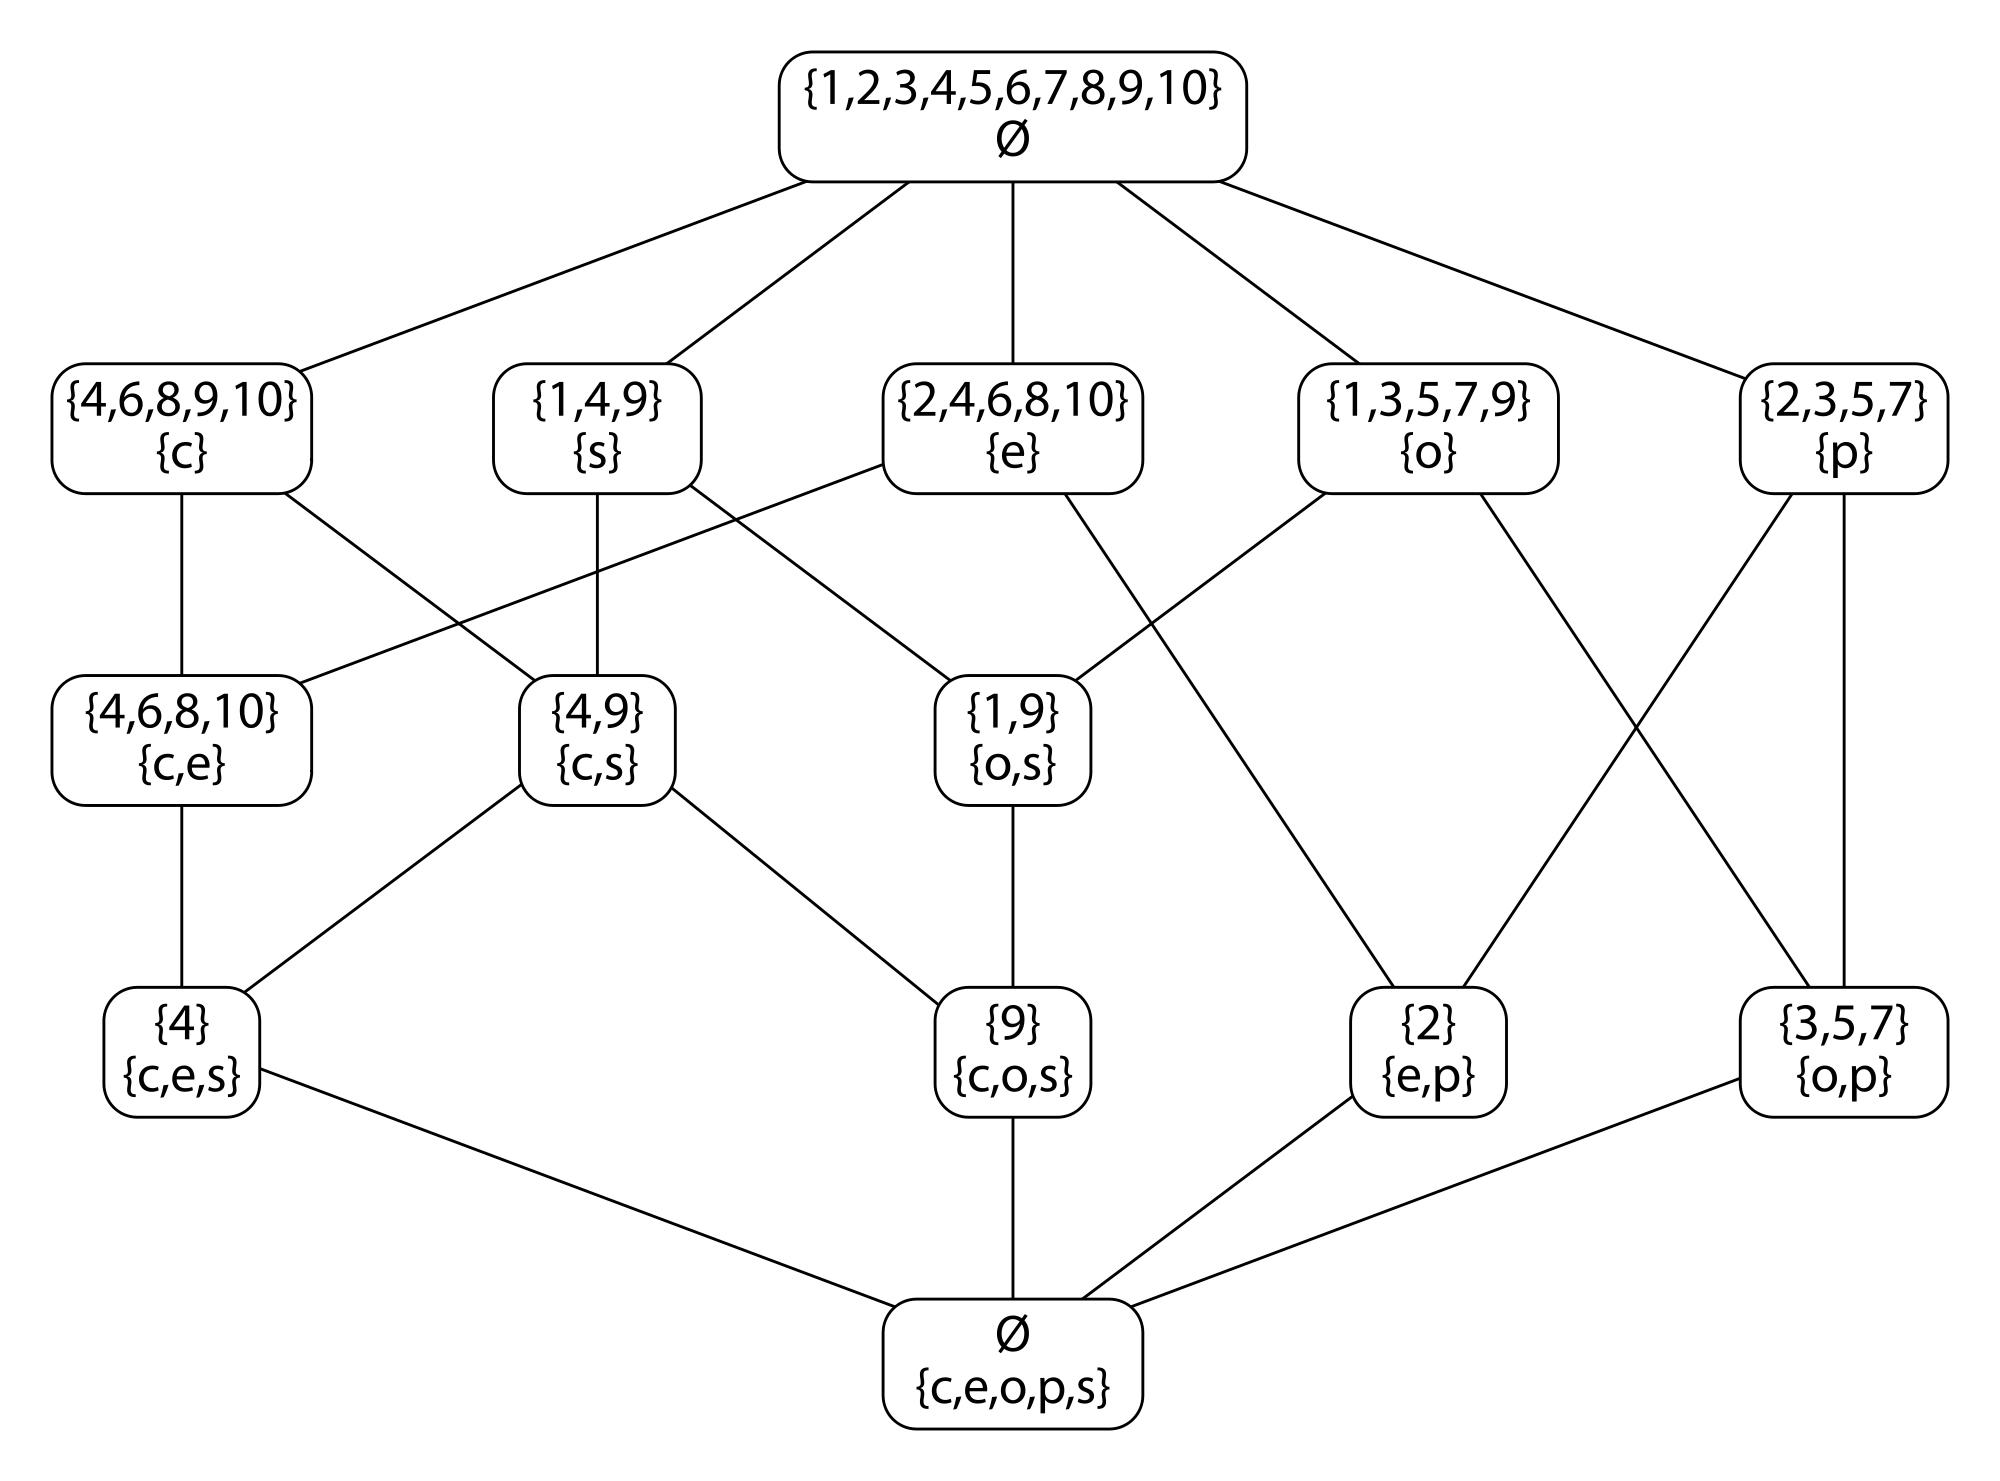
\includegraphics[width=\linewidth]{./images/fcaExample}
\caption{Hasse diagram, with the integers 1 to 10 as objects and attributes square (s), prime (p), composite (c), even (e), and odd (o)}
\label{figure:example}
\end{figure*}

A Hasse diagram is a graph where the vertices represent formal concepts and edges represent the relation $\le$ among the formal concepts. An edge between formal concepts $C_i$ and $C_j$ is drawn, when $C_i \le C_j$ and there does not exist a formal concept $C_x$ such as $C_i \le C_x \le C_j$. To increase the readability, the nodes are ordered in layers. The concepts in top are more general, the concepts in the bottom are the more specific. There are two special concepts: supremum and infimum. The supremum is vertex node in the top and the attributes in its intent are those which are present in all objects. In most cases its intent is empty. The infimum is the vertex in the bottom and the objects in its extent are those which have all attributes. In most cases its extent is empty.\\

After this general introduction, we will describe in the next section how we can apply \acrshort{fca} to \acrshort{ir}.

\subsection{Application of \acrshort{fca} in \acrshort{ir}}

The examples depicted in table \ref{table:example} and figure \ref{figure:example} are only exemplary. How did \acrshort{fca} affected the real world? According to Poelmans et al. has been \acrshort{fca} "applied in many disciplines such as software engineering, knowledge discovery and \acrshort{ir}" \cite{Poelmans2013} and they did two comprehensive surveys on the application of \acrshort{fca} \cite{Poelmans2013, Poelmans2013b}. \\

Carpineto et al.\cite{Carpineto2005} describe the start of \acrshort{fca} in \acrshort{ir}:

\begin{quote}
In the 80's, basic ideas were put forth - essentially that a concept can be seen as a query (the intent) with a set of retrieved documents (the extent) and that neighbor concepts can be seen as minimal query changes."
\end{quote}

This means that the objects are documents and the documents are treated as a set of words. An attribute means that a word occur in this documents. In this simple form, this has a major drawback because it is not possible to we weight terms or for instance to rank among documents with same attributes.\\

The different algorithms to create concept lattes or an in-depth analysis of \acrshort{fca} for text mining are not covered in this thesis. The interested reader is guided to study the work from Carpineto and Romano \cite{carpineto2004concept} for a detailed investigation. \\

The visual representation of of those \acrshort{ir} systems is discussed in the related work section \ref{Related Work}. Before we do this, let us get to know some principles of interface design. \\

\section{Interface Design}
\label{id}

The interaction from the user with the system is what exactly matters to the user. The interaction of humans with computers has its own research area, human-computer interaction, and one of its pioneers is Ben Shneiderman. In the following, two principles from him will be presented: The "Eight Golden Rules of Interface Design" and the "Visual Information Seeking Mantra".

\subsection{Eight Golden Rules of Interface Design}

This rules are genreal advices for user interface designers which should apply to all interfaces. Ben Shneiderman et al. present this rules in their book \cite{Shneiderman2010}. The rules are names and explained with my own remarks. \\

\begin{itemize}
	\item Strive for consistency: Use similar actions in similar situations. Use identical terminology, colors, fonts etc. throughout the system.	
	\item Cater to universal usability: Design for the needs of a diverse user group (skill level, age, gender and others)
	\item Offer informative feedback: Give system feedback for every action.
	\item Design dialogs to yield closure: Sequences of actions should be grouped. Give feedback on completion of a group.
	\item Prevent errors: Design the system that the user cannot even do errors in the first place. But if she does some, offer instructions how to recover.
	\item Permit easy reversal of actions: Actions should be undone. This gives the user confidence to explore the system.
	\item Support internal locus of control: The user should think that she is in charge of control.
	\item Reduce short-term memory load: Reduce the number of things the user has to keep in mind while using the system.
\end{itemize}

As you can see, the rules are open to interpretation. There exits alternative principles for instance: Donald Norman's Design Principles \cite{Norman2013} or Jakob Nielsen's "10 Usability Heuristics for User Interface Design" \cite{Nielsen1995}. \\

This principles can be applied to all user interfaces. In the next section, design principles will be presented where the user views a large collection of items.

\subsection{Visual Information Seeking Mantra}

The visual information seeking mantra (the Mantra) was introduced by Ben Shneiderman \cite{Shneiderman1996} and are based on his experience with past projects. Albeit the Mantra was intended to be a "descriptive and explanatory" \cite{Card1999}, "in effect, the Mantra has become a prescriptive principle for many information visualization designers", write Craft and Cairns \cite{Craft2005}. \\

The Mantra describes user interface design principles for systems when the "users are viewing collections of items, where items have multiple attributes" \cite{Shneiderman1996}. The starting principles are: overview first, zoom and filter, and then details on demand. They will be explained below and added by three other principles. \\

\begin{itemize}
	\item Overview: Gain an overview of the entire collection.
	\item Zoom: Zoom in on items of interest.
	\item Filter: Filter out uninteresting items.
	\item Details-on-demand: Select an item or group and get details when needed.
	\item Relate: View relationships among items.
	\item History: Keep a history of actions to support undo, replay, and progressive refinement.
	\item Extract: Allow extraction of sub-collections and of the query parameters.
\end{itemize}

Some task needs more explanation which I will give in the following with help from related literature.

\subsubsection{Zoom and Filter}

This task are responsible for reducing the complexity of the data collection. 'Zoom' means that the user focuses on items she wants to see. 'Filter' means that she can hide items which are not interesting for her.

\subsubsection{History}

It is important to give the user the possibility to easily recover from mistakes or loss of interest. In addition, "it is rare that a single user action produces the desired outcome. Information exploration is inherently a process with many steps, so keeping the history of actions and allowing users to retrace their steps is important." writes Shneiderman \cite{Shneiderman1996}.

\subsubsection{Extract}

Once interesting objects are found, the user should have the possibility to extract them from the system. Shneiderman describes printing, emailing or saving the item to the disk as 'extraction'.

\subsection{Final Remarks}

The presented ideas are based mostly on the experience of one person: Ben Shneiderman. The huge number of citations show that his work is influential for a lot of people. But this is not real science. Craft and Cairns \cite{Craft2005} are calling for empirical justification of the Mantra. This is an indication that human-computer interaction is only at the start point - there is a still a lot of research to do. \\

In addition, you have to interpret this rules and adapt them to the current situation. Furthermore, there overall humans are involved, a very complex system which is hardly explored.

\chapter{Related Work} \label{Related Work}

After introducing formal concept analysis in section \ref{Formal Concept Analysis}, let us review and discuss related work. In the first three sections, we go over a lot of different \acrshort{fca}-based approaches. Eventually, we evaluate one \acrshort{fca}-based real world application in detail in regard to the interface design principles described in section \ref{id}. In section \ref{dyafs}, a non-\acrshort{fca} based approach is shown which is very related to \acrshort{fca}: \acrshort{dt} and Faceted Search. \\

\section{Full Hasse Diagrams}

The traditional, static visualization of concept lattices are Hasse diagrams as describes in section \ref{Formal Concept Analysis}. They are also named \textit{line diagrams}. Eklund et al. \cite{Eklund2004} conducted user studies and proclaim that non-FCA-experts can read Hasse Diagrams if you fine-tune the Hasse diagram. For instance by choosing appropriate colors, making us of symbols and carefully positioning the vertices in layer. \\

But in the domain of \acrshort{ir} on documents you get formal contexts with a lot of objects. Those Hasse diagrams scale bad for large concepts lattices. Kuznetsov et al. \cite{Kuznetsov20072}  describe this resulting visualization: "Representing concept lattices constructed from large contexts often results in heavy, complex diagrams that can be impractical to handle and, eventually, to make sense of." Especially the high connectivity of the graph results in enormous edge crossing. The image \ref{figure:firstVisualizaion} shows the first results from data in the digital humanities project. The software XX was used. \\

\begin{figure*}[!ht]
	\centering
	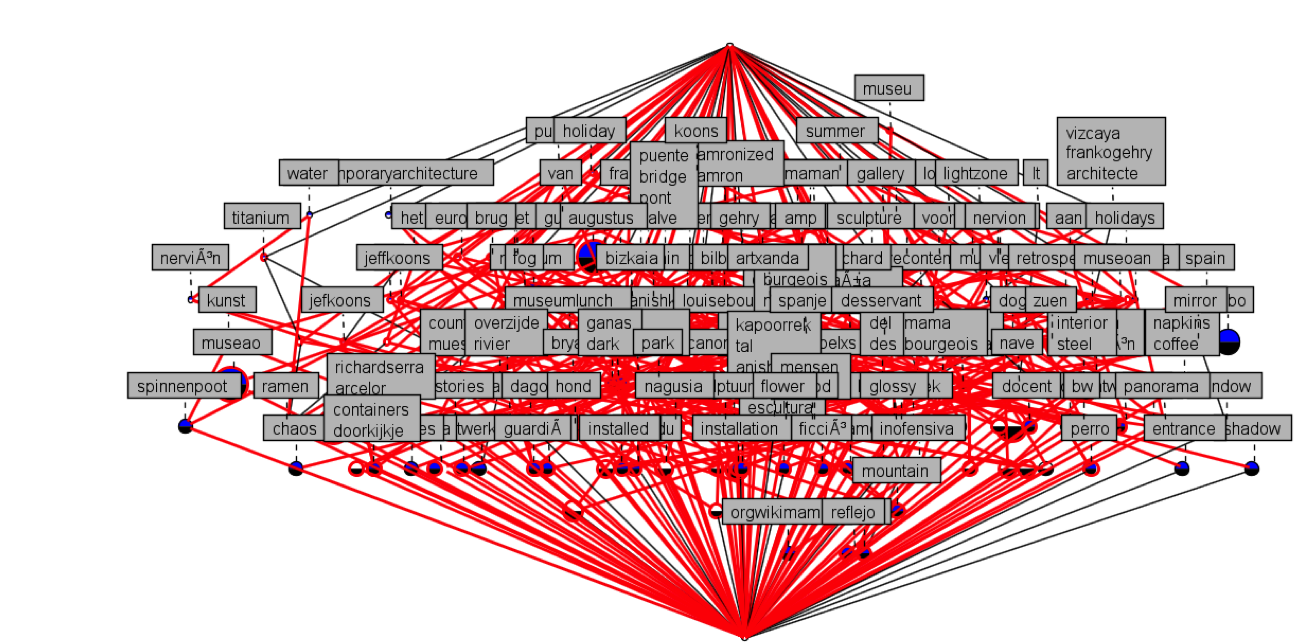
\includegraphics[width=\linewidth]{./images/firstVisualization}
\caption{First visualization of digital humanist data with traditional \acrshort{fca} software}
\label{figure:firstVisualizaion}
\end{figure*}

The visualization is useless. What can be done to improve the situation? The Hasse can be pruned by reducing the number of vertices. The different techniques are discussed in the next section.

\section{Pruned Hasse Diagrams}

\subsection{Reduce Number of Formal Concepts}

One way to reduce the number of vertices is to compute the \textit{iceberg lattices} as described by Stumme et al.\cite{Stumme2002}. They result after the application of a data mining technique "frequent item-set mining" from Agrawal et al.\cite{Agrawal1993}. Only formal concepts are selected which are considered 'frequent'. A formal concept is frequent if its intent, the set of attributes, is frequent. Let $B$ be the intent and $minSupport \in [0, 1]$, then $B$ is frequent if $ |B'|/|G| \geq minSupport$. This means the attribute set has to specify a high portion of objects; at least $minSupport$. \\

 This approach has some drawbacks as Kuznetsov et al. \cite{Kuznetsov20072} point out: "One should be careful not to overlook small but interesting groups, for example, “exotic” or 'emergent' groups not yet represented by a large number of objects, or, groups that contain objects who are not members of any other group." They propose to only select 'stable' concepts and write "A concept is stable if its intent does not depend much on each particular object of the extent." \cite{Kuznetsov20072}. It is also possible to apply traditional cluster techniques like fuzzy K-Means clustering to \acrshort{fca} \cite{AswaniKumar2010}. \\

	While all these techniques undoubtable reduces the number of formal concepts, it is to question if the results are any helpful. In our case of \acrshort{ir}, we apply \acrshort{fca} to explore the data and get insights about the lattice structure. When pruning the nodes, you are losing many data relationships, many formal concepts and, consequently, the "power" of \acrshort{fca} as exploratory technique is significantly reduced. When we deal with large concepts lattices, the number of nodes has to be very low if we want to represent them with Hasse diagrams. In the year 2015, the question is not how can I visualize and analyze 16 formal concepts as in figure \ref{figure:example} - it is more how can I analyze 160000 formal concepts. For this tasks, this approach is not appropriate. \\
	
	But this reduction techniques can be useful to reduce the clutter in the lattice. They can be used in combination with our visualizing techniques as described in the upcoming section \ref{Local View}. \\
	
\subsection{Nest Formal Concepts}	

Another idea are \textit{nested line diagrams} - line diagrams are another name for Hasse diagrams. All attributes of a formal context are partitioned into layers. For instance if you just have two layers. For the first layer: built up the Hasse diagram with the attributes of the first layer. For each vertex in the resulting Hasse diagram, built up a Hasse diagrams \textit{inside} the vertex. This secondary Hasse diagrams are built from the objects in each vertex (extent of the formal concept). This can be done for an arbitrary number of layers. An example from Carpineto and Romano \cite{carpineto2004concept} is shown in figure \ref{figure:nested}. The general idea should be clear without explaining the context - if not Carpineto and Romano \cite{carpineto2004concept} describe it more in detail. \\

\begin{figure*}[!ht]
	\centering
	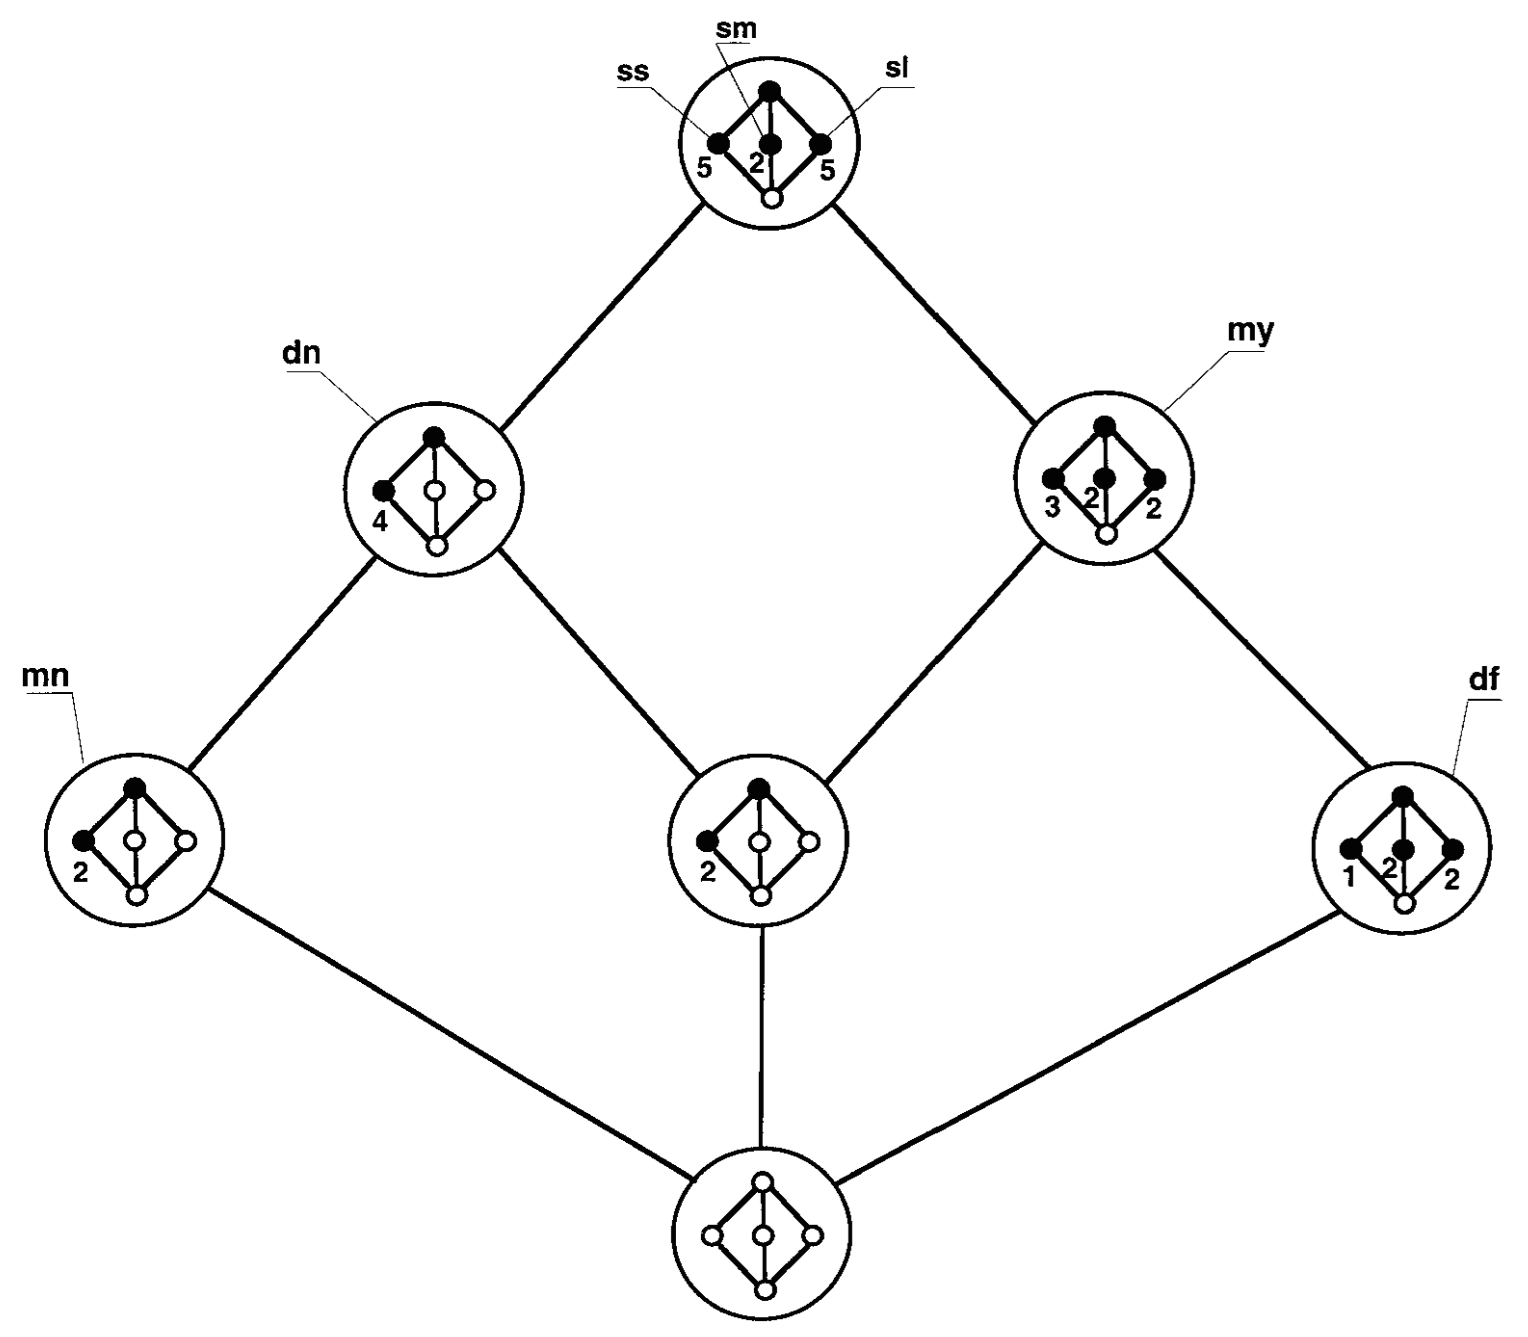
\includegraphics[width=0.5\linewidth]{./images/nested}
\caption{Nested line diagram}
\label{figure:nested}
\end{figure*}
	
But how to partition the attributes? You have to select them manually. If you have an taxonomy of the attributes you can make use of them. In the case of text mining we do not have an taxonomy and thereby cannot make use of it. Furthermore: \acrshort{fca} is good at building relationships with arbitrary attributes. If you have a taxonomy, there are way better techniques one will be presented in section \ref{dyafs}: "Dynamic Taxonomies and Faceted Search". \\

\section{Local View}
\label{Local View}

Instead of showing the full Hasse diagram, the user can see a local view on the lattice. We will give an overview about the basic idea and applications before we review one real-world application in detail. \\

One could argue that you just have to visualize everything and then allow to zoom on nodes. This techniques is common among network visualizations \cite{Herman2000}. But because of the high connectivity of the graph, this is not helpful to Hasse diagrams. You can see this at the tool 'FCART' presented by Neznanov and Parinov \cite{Neznanov2014}. In figure \ref{figure:fcart} they visualize a concept lattices comprising more than 20000 concepts. Without going into detail and without arguing the general appearance of the user interface we can see, that this kind of approach is doomed to fail. Furthermore, this procedure takes a lot of computation power. \\

\begin{figure*}[!ht]
	\centering
	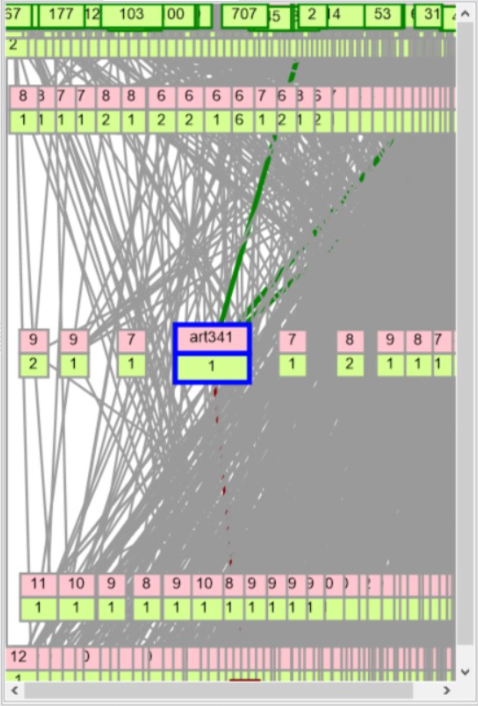
\includegraphics[width=\linewidth]{./images/fcart}
\caption{FCART visualizing concept lattice with over 20000 concepts.}
\label{figure:fcart}
\end{figure*}

Let us review other, more successful approaches. \\

\subsection{Introduction}

There exist a lot of different names for a similar approach. Eklund et al. name it \textit{conceptual neighborhood}\cite{Eklund2009,Eklund2012} and Carpineto and Romano name it \textit{hybrid navigation} \cite{Carpineto1996}. But there share the same ideas: the interface is always focused on exactly \textit{one} formal concept. The user can navigate through the lattice by going up (becoming more general) or going down (becoming more special). In the context of \acrshort{ir} this means removing terms or adding terms. They also offer the possibility to query the system with a search. In most cases, the user would start with a search and if there exist a corresponding formal concept it focuses on it. Then the user can fine-tune the search. The idea originated from the \acrshort{ir} field and was first proposed by Godin et al. \cite{Godin1989}. \\

Two underlying information seeking models stand behind his approach. First, user tend to start with a short query and then refine their needs. Hearst \cite{Hearst2009} write  while referring to \cite{Marchionini2006,Bates1990}:
\begin{quote}
	A commonly-observed search strategy is one in which the information seeker issues a quick, imprecise query in the hopes of getting into approximately the right part of the information space, and then doing a series of local navigation operations to get closer to the information of interest
\end{quote}

Second, it easier for the user to choose from suggestions than to formulate a query. Aula writes \cite{Aula2005}:
\begin{quote}
	Considered in cognitive terms, searching is a more analytical and demanding method for locating information than browsing, as it involves several phases, such as planning and executing queries, evaluating the results, and refining the queries, whereas browsing only requires the user to recognize promising-looking links.
\end{quote}

Third, the incremental navigation prevents the user from getting empty result lists. This is related to the design principle from Shneiderman: Prevent the user from making mistakes. But they can still fail when they then search. \\

Godin et al. \cite{Godin1993} evaluated their work in comparison to boolean retrieval and hierarchical retrieval and proclaim that "[their experiment] suggests that retrieval using a Galois lattice structure may be an attractive alternative since it combines a good performance for subject searching along with browsing potential." Galois lattice is a synonym for concept lattice.\\

\subsection{Applications}

Carpineto and Romano picked up the idea from Godin et al. and developed a \acrshort{fca} search engines ULYSSES \cite{Carpineto1995,Carpineto1996}. The user can fine-tune what neighboring vertices are displayed by bounding the information seeking space. They are not only showing directly adjacent vertices but also vertices that do not exceed a given distance. It is also possible to restrict the space to vertices which are above, below, left or right of the focus. In figure \ref{figure:ulysses} is a screenshot of the system. \\

\begin{figure*}[!ht]
	\centering
	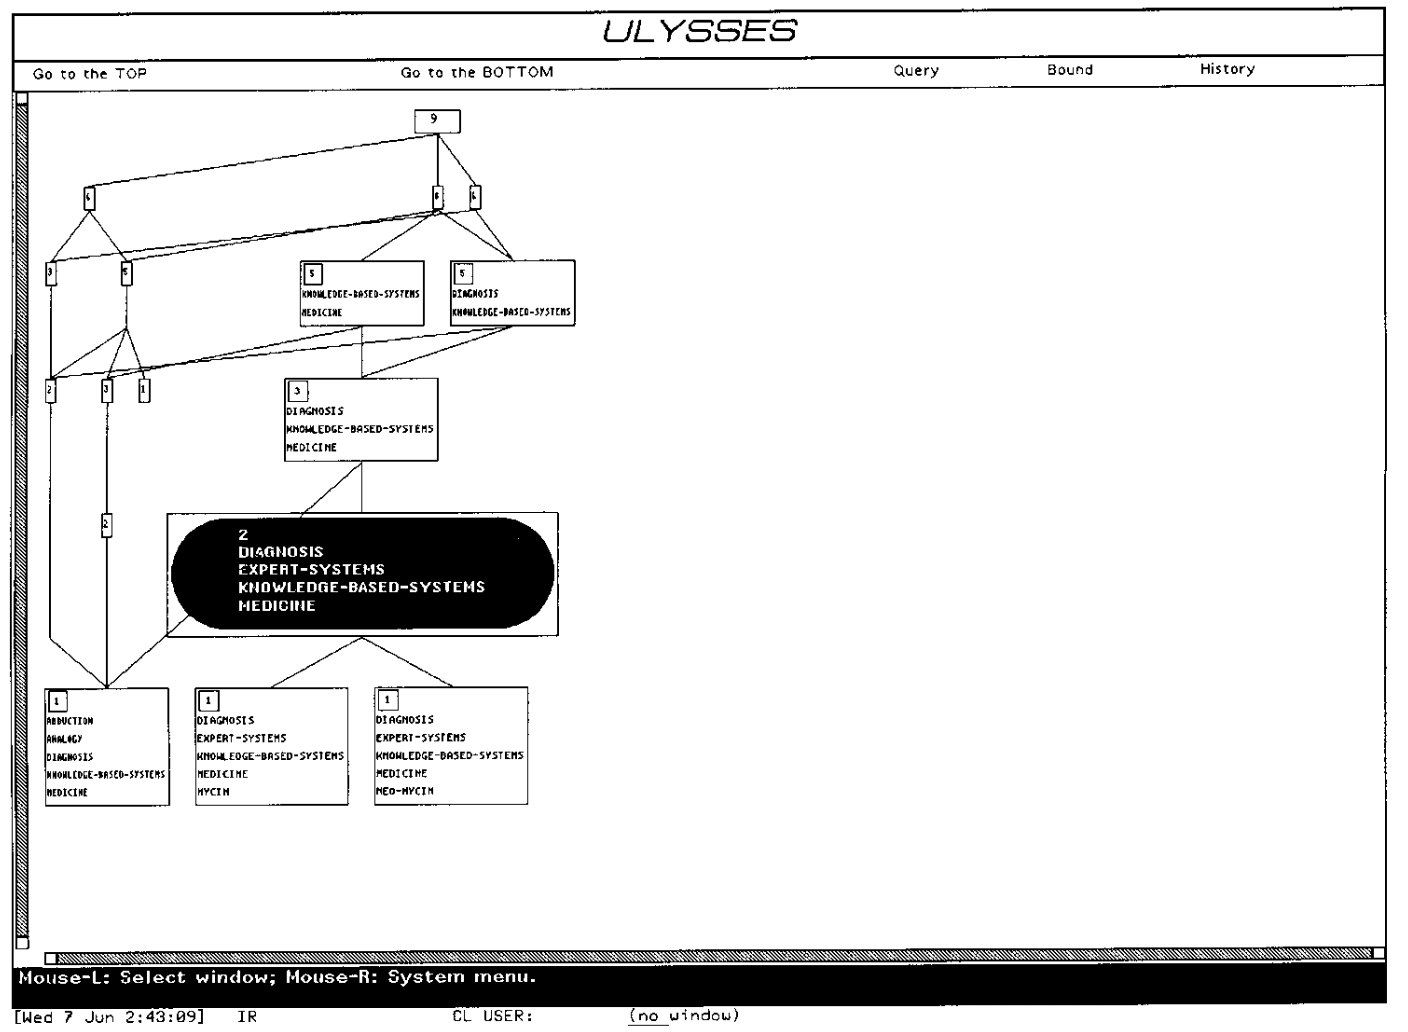
\includegraphics[width=\linewidth]{images/ulysses}
\caption{ULYSSES with focus on the black node \cite{Carpineto1996} }
\label{figure:ulysses}
\end{figure*}

In their following work, CREDO \cite{Carpineto2004}, Carpineto and Romano followed the look of ordinary search engines. The presentation of the concept lattice is not oriented at the Hasse Diagram. It looks more like a folder structure. Shown in \ref{figure:credo}. Work that is similar comes from Koester \cite{Koester2006}, Dau et al.\cite{Dau2008}, Nauer and Yannik \cite{Nauer2009} and Cigarran et al. \cite{Cigarran2004}. In all this cases, the concept lattice is built on the fly from the result list of search engines. This come with special interest like performance which is not inserting to us. And it is - again like many \acrshort{fca} application - restricted to relatively small number of formal concepts. Let us move on to some application of \acrshort{fca} to document collections. \\

\begin{figure*}[!ht]
	\centering
	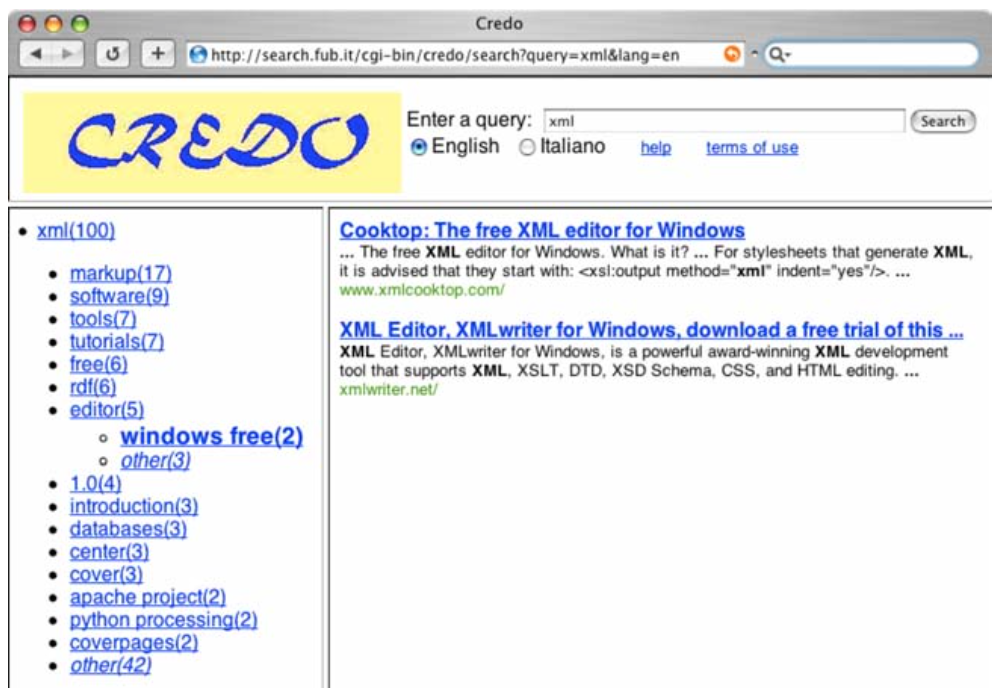
\includegraphics[width=\linewidth]{images/credo}
\caption{Screenshot of CREDO, after query 'xml' and browsing after 'editor(5)' and 'windows free(2)' \cite{Carpineto2004} }
\label{figure:credo}
\end{figure*}

Eklund et al. applied \acrshort{fca} to email organization\cite{Eklund2004}, image browsing \cite{Ducrou2006,Ducrou2008} and a later work is the 'Virtual Museum of the Pacific' \cite{Eklund2009,Eklund2012}. Let us review this museum because: it visualizes a static documents collection as we do and it is a rare example of \acrshort{fca} outside academia. It is also web-based like our desired interface. It was created after doing a lot of research into his field. It was built in 2000 - so it is fairly recent. They conducted a usability study with museum experts and non-experts. \cite{Eklund2012}

\subsection{Virtual Museum of the Pacific}
 
The museum was created to give user the possibility to browse images of museum objects. It is available on the web \footnote{\url{http://epoc.cs.uow.edu.au/vmp/} - Credentials are required. Use username: filter and password: 45755} and it is advised to take a look at it before continue reading. \\

\begin{figure*}[!ht]
	\centering
	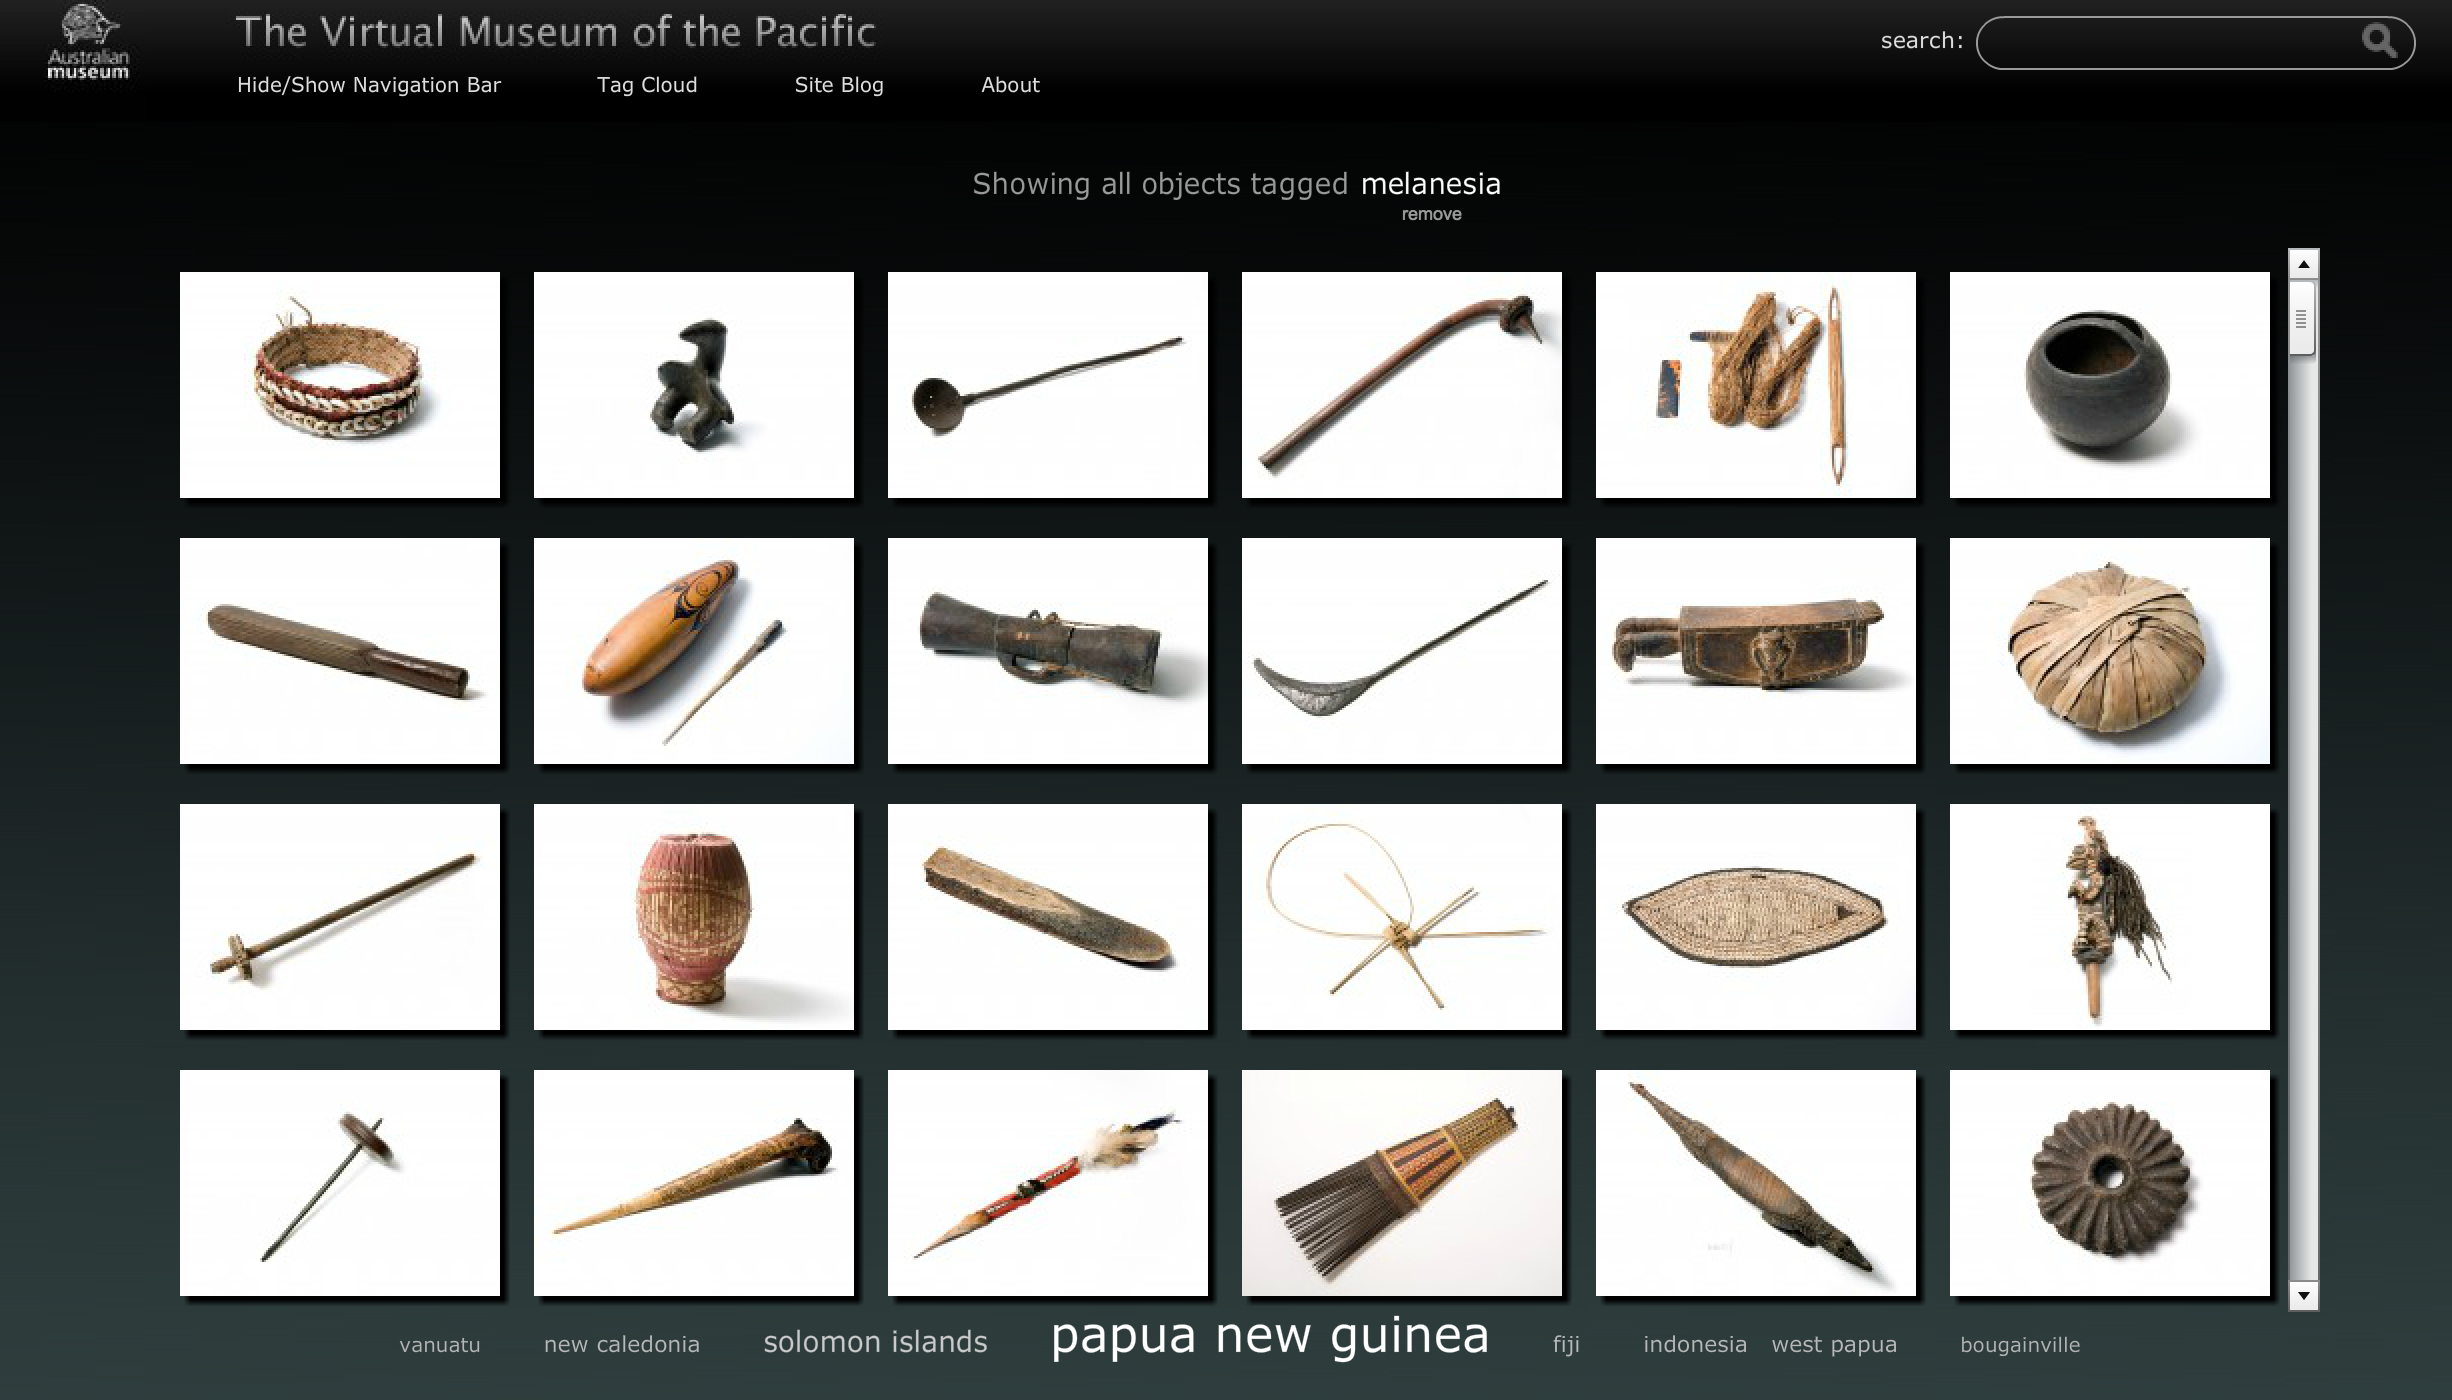
\includegraphics[width=\linewidth]{images/pacific}
\caption{The Virtual Museum of the Pacific, focus on concept 'melanesia'}
\label{figure:pacific}
\end{figure*}

After the login it is not clear where to start. If you are completely new to the topic, it is a good idea to start with the word cloud. Here comes the Mantra into play: Overview first - details on demand. No real overview is given, this might confuse user. \\
 
 The interface sets the objects in he focus of the interface. This is, in my opinion, a good decision. The user is probably more interest in the object than on the structure which was built around the objects (the lattice). \\
 
 Above the objects is the current intent of the formal concept shown. It is possible to remove terms from the current selection to generalize. Below the objects are terms suggested to specify the information needs. When the user clicks on the term the view changes with the newly added item. The sidebar categorizes the attributes/terms and it possible to filter out uninteresting concepts. This categorization contradicts the whole purpose of \acrshort{fca} but might help the users. \\
 
 To get details on demand, you have to click on an item. From there you can also find related items. \\
 
 It is possible to search but this search is very rudimentary. It is very easy to implement a type ahead (autocomplete/suggestion/autofill) for static data set. This is a real problem and there is no excuse not to stick to well-proven user search interface principles as described by Hearst \cite{Hearst2009}. \\
 
 The biggest problem with the his interface is the missing home/reset button and the absence of any form of history. As Shneiderman \cite{Shneiderman1996} pointed out "Information exploration is inherently a process with many steps, so keeping the history of actions and allowing users to retrace their steps is important." \acrshort{fca} is a exploratory technique. Not implementing \textit{any} possible to go back is a utter failure. You can this in the evaluation as they point out \cite{Eklund2012}: "Users also had difficulty understanding the notion of conceptual navigation as a way of navigating an information space, rather than a fixed hierarchy with a well defined ‘home’ state." and "[..] many users felt ‘lost’ within [the FCA-based] style of navigation. A recommendation was put forward so that users could at least back track through the navigation sequences (in the form of a ‘Back’ button) or that users could easily go back to a ‘home’ or ‘reset’ state." They are not going to discuss this problems - even thought the navigation is \textit{the} important problem with FCA. They defend their failure with unfamiliarity of the users \cite{Eklund2012}: "there were a number of common issues, mostly relating to the unfamiliarity of the interface". This is not a real argument because the users are always unfamiliar with new interfaces. \\
 
  Combined with meaningless quotes from participants \cite{Eklund2012} : "There should be more of this kind of thing, but there’s room for improvement" or "I think it’s really good—it gives specialized information." and a weak summary \cite{Eklund2012}:
  \begin{quote}
  "Overall, the study concludes that conceptual based browsing can offer significant merit for browsing Pacific collections, and that by resolving the identified issues, the core functionality of searching and browsing via \acrshort{fca} can be considerably easier for users to learn and engage with." 
  \end{quote}
  (Easier than what? There was NO comparison with other IR techniques in the whole study) this paper leaves a bitter aftertaste. It started with a good idea but the implementation - in my opinion - is a complete failure. Instead of blaming the stupidity of the users, they should have looked at their own mistakes and learned from them.\\
 
\subsection{Conclusion}

While \acrshort{fca} is famos in the academic stuff it does not really help the world at all. There exist only a few useful examples and most of them were conducted on small lattices. Focusing on formal concept on only showing neighboring nodes is the way to built interfaces. Before describing the idea of my interface in detail, let us review some related techniques which is similar to \acrshort{fca} and go into the industry. Feel free to skip this section and go straight to section XX.

\section{\acrlong{dt} and Faceted Search}
\label{dyafs}

Sacco and Tzitzikas \cite{Sacco2009} write: "Although \acrshort{fca} and \acrlong{dt} are apparently two distinct approaches to information modeling and access, and they use a different terminology, they are closely related". Completely introducing  \acrlong{dt} (\acrshort{dt}) would exceed this thesis. The interested reader is guided to study the work from Sacco and Tzitzikas \cite{Sacco2009}. \\

 The whole point of this section is to deconstruct a techniques which is called \textit{conceptual scaling}\cite{carpineto2004concept}. The technique is applied to many-valued data sets to change them into single-valued data sets. \acrshort{fca} only knows single-valued data sets. Let us take a look at table \ref{table:manyvalued}. \\

\begin{table}[h]
\caption{many-valued data set}
\label{table:manyvalued}
\centering

\def\arraystretch{1.2}% 
\begin{tabular}{ c c c }
\hline
 Name & Age & Hometown \\
\hline
Johannes & 24 & Schwerin \\
Ana & 35 & Madrid \\
Peter & 47 & Magdeburg \\
\hline
\end{tabular}
\end{table}

The objects are human beings and they are categorized by the attributes name, age and hometown. With conceptual scaling  the attributes for the object Johannes are: "Name\_Johannes", "Age\_24", "Hometown\_Schwerin" and correspondingly for the other people. Now we have only a single-valued data-set which is needed for \acrshort{fca}. \\

But this method, albeit it is widespread, is, at least for IR, problematic. From a user-centered perspective, complexity reduction is the key point. How do we break massive, complex data set down to make them understandable for the users? So this transformation sounds like a contradiction - and it is. Zobel describes this kind of research as follows:

\begin{quote}
Much research — far too much — is just misguided. People investigate problems that are already solved and well understood, or solve problems that technology has made irrelevant, or don’t realize that the proposed improvement actually makes the method worse.
\end{quote}

So for many-valued data, \acrshort{fca} is not a appropriate technique. The use of facet search is shown in figure \ref{figure:flamenco}. \\

\begin{figure*}[!ht]
	\centering
	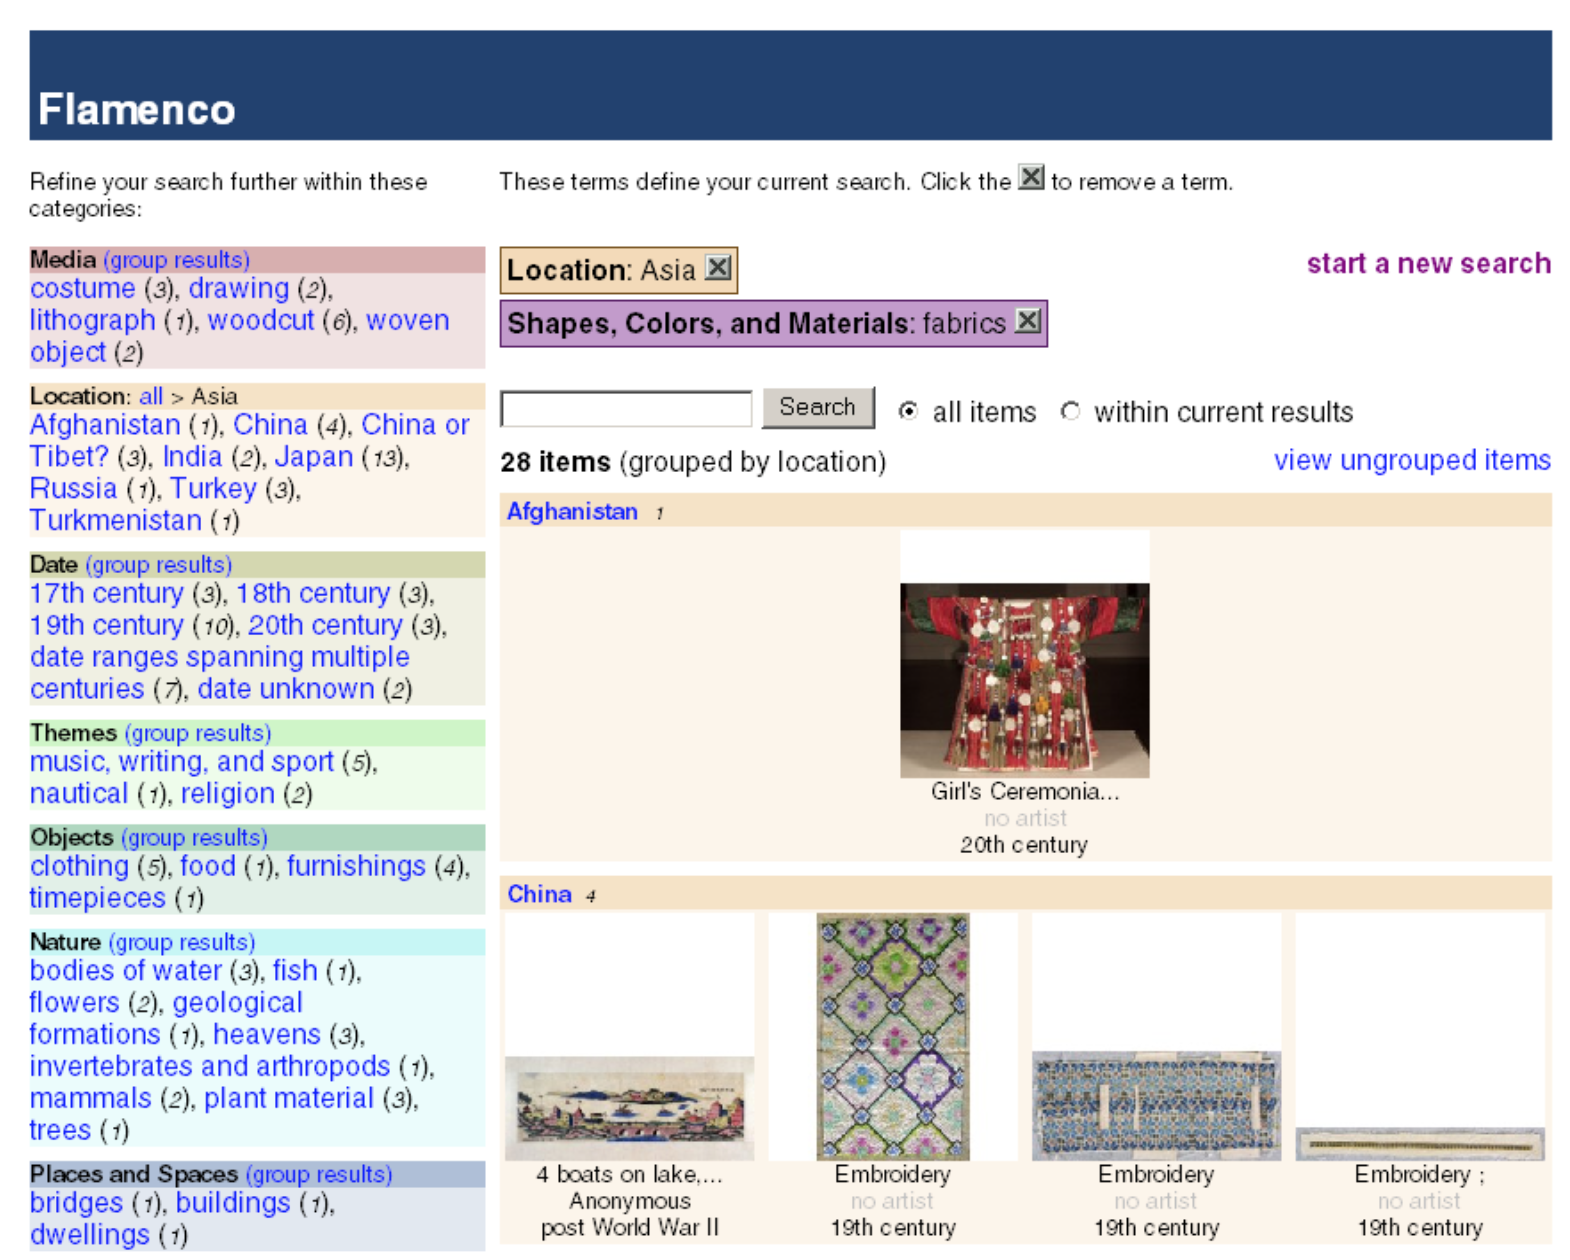
\includegraphics[width=\linewidth]{images/flamenco}
\caption{Flamenco with ongoing focus}
\label{figure:flamenco}
\end{figure*}

You can see that the search is currently narrowed down be restricting location to 'Asia' and Shapes etc. to 'fabrics'. It is possible to continue becoming more specific by choosing attributes and value from the sidebar on the left. Or becoming more general by removing current choices. It is very similar to the local view of \acrshort{fca} described in section \ref{Local View}. Sacco and Tzitzikas \cite{Sacco2009} compare \acrshort{dt} to \acrshort{fca}:
\begin{quote}
DT is less informative, but it ensures the results displayed to users is manageable because they are expressed in terms of the original taxonomy. This reduces the cognitive effort of users and is a simpler and more intuitive representation than the line diagrams generally used in \acrshort{fca}.
\end{quote}

To summarize the use for IR: Use \acrshort{dt} if you have many-value datasets and \acrshort{fca} for single-valued datasets. Let us continues the design of the application of the system.

\chapter{Fancy \acrshort{fca} 1.0}
\label{Fancy 1.0}

We describe the idea inferred from discussing related work in section \ref{Related Work}. Then we describe the implementation of the frontend followed by the backend.

\section{Idea}

The general idea comes from the digital museum but we identified the weaknesses and make it better. \\

\begin{figure*}[!ht]
	\centering
	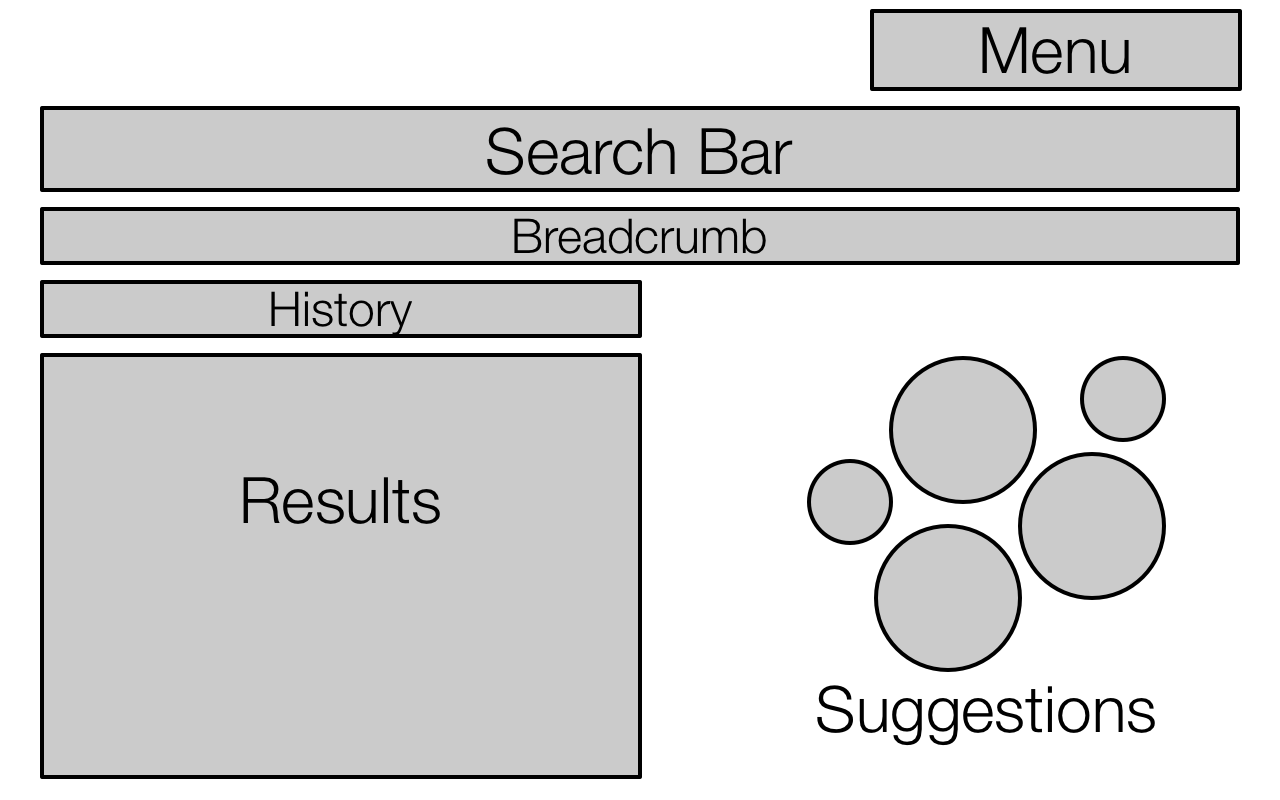
\includegraphics[width=\linewidth]{images/schema}
\caption{The Interface}
\label{figure:schema}
\end{figure*}

First, the search interfaces did not followed any design principles. The interface should remind users of modern search engines: Search bar on top vertical result list bottom. Each result has a title withs links to the original page of the map. A snippet is shown with highlighted words from the query. We could not provide thumbnails of the maps because we did not had access to the pictures itself. It was planned to add this feature in later iterations. \\

Second, there was a lack of history of actions or at least orientation. For this we have two functionalities: Breadcrumbs and Navigation History. Breadcrumbs save the current path of search and allow it to go easily pack. The navigational history allows more possibilities to backtrack. If the user is logged in, it save the history forever. If she is not logged in, it only saves the session history. \\

Third, the user can save documents which she found interesting. \\

Fourth, if the user is logged in, all actions are logged and send to the server. This was to evaluate the user behavior. \\

Fifth, the neighboring concepts ( the 'suggestions') are shown right next to the results as a word cloud. The words are presented in a bubble. The font size and bubble radius depend on the documents which are presented in there.

\begin{figure*}[!ht]
	\centering
	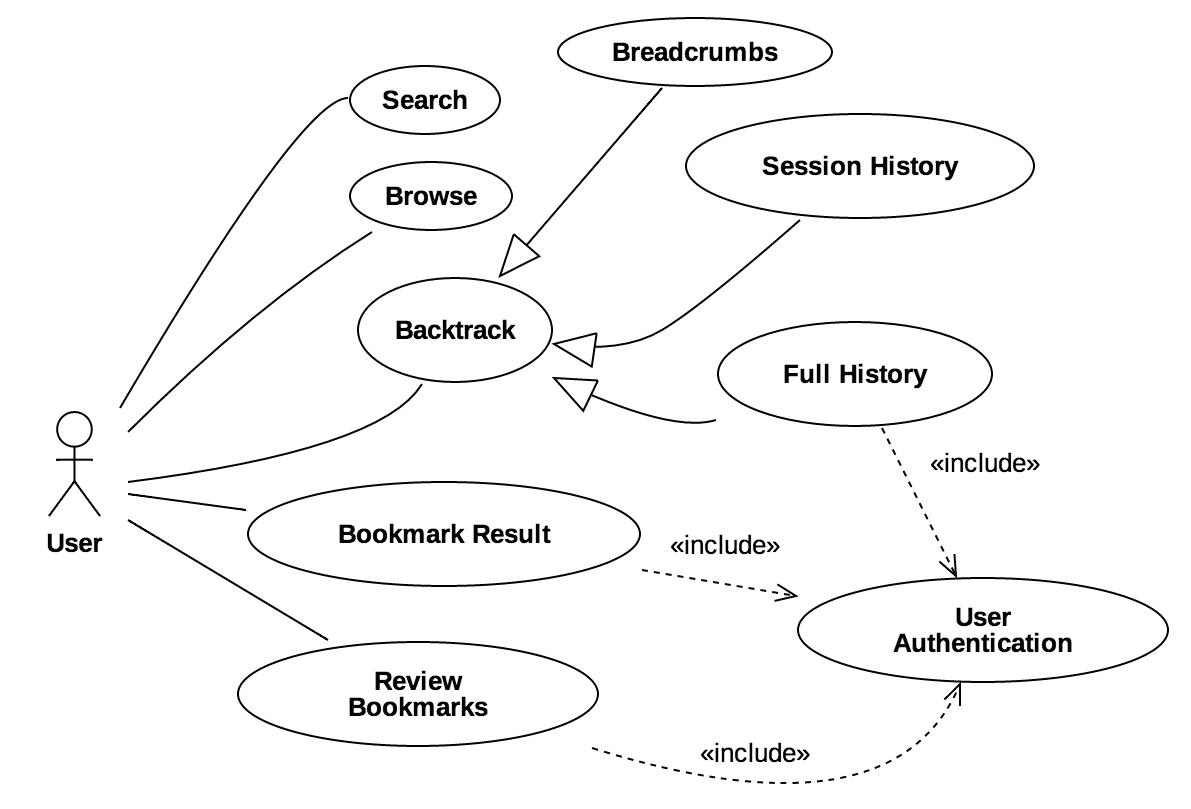
\includegraphics[width=\linewidth]{images/usecase}
\caption{The Interface}
\label{figure:usecase}
\end{figure*}

\section{Frontend}

The interface was implemented with web techniques. So HTML, CSS, Javascript. Instead of writing pure HTML, we use the Jade templating engine \footnote{\url{http://jade-lang.com}}. Instead of writing Javascript, we use CoffeeScript \footnote{\url{http://coffeescript.org}} which compiles to Javascript but offers semantic sugar. For the the word cloud I use D3\footnote{\url{http://d3js.org}} \cite{Bostock2011} as background. D3 utilized SVG to draw elements which are also accessible via the DOM API. The word cloud is a customized graph force-directed layout based on the work from Vallandingham \cite{Vallandingham}. Bootstrap\footnote{\url{http://getbootstrap.com}} gives the overall good look to the site.

\section{Backend}

For the backend, Node.JS with the Express Framework \footnote{\url{http://expressjs.com}} was chosen. Reason one, it is good at handling multiple request in parallel. Reason two, I can use the same programming language for frontend and backend: Javascript (CoffeeScript). For data we use MySQl as database because it was already installed on the server. But we use an ORM, Sequelize \footnote{\url{http://sequelizejs.com}},  so you can easily change the database.

\section{Disccusion}

The whole implementation has one problem: The data is provided as a JSON file. The clients loads the whole file in the beginning. All the navigation happens in the front end. While it a good thing, that during the navigation the client does not have to talk with the server, it is a problem that the client has to deal with over 80 megabytes of data. The server compress the JSON file to eight megabytes to make the time to download it okay. But it may only run on powerful computers with sufficient RAM because the browser will consume a lot of it. The design decision was taken before it was clear that the JSON file would be so huge. In the beginning it was under ten megabytes. \\

That the thumbnails of the maps are not presented is a problem. Albeit all the analysis was done on the metadata, a visual representation would be very useful.

\chapter{Evaluation}
\label{Evaluation}

The design of an interface is highly subjective. User studies can help to evaluate an interface but computer scientists are not experts in human studies. For this, a brief review of different techniques for human studies is given first. Then we describe the setup of the study, describe the results and finally conclude. \\

\section{Background}

We will only scratch the surface here. A comprehensive introduction into "Methods for Evaluating Interactive Information Retrieval Systems with User" gives Kelly \cite{Kelly2007}. A shorter introduction gives Hearst in her book on "User Search Interfaces" in Chapter 2. \cite{Hearst2009}.\\


\subsection{Introduction}

So we want to measure usability, but how is it defined? The ISO 9241-11, 1998 \cite{ISO} defines three aspects of usability:
\begin{itemize}
	\item Effectiveness: Accuracy and completeness with which users achieve specified goals.
	\item Efficiency: Resources expended in relation to the accuracy and completeness with which users achieve goals.
	\item Satisfaction: Freedom from discomfort, and positive attitudes towards the use of the product.
\end{itemize}

\subsection{Experiment vs. Evaluation}

It is important to distinguish between the terms 'experiment' and an 'evaluation'. Kelly \cite{Kelly2007} writes:
\begin{quote}
"Evaluations are conducted to assess the goodness of a system, interface or interaction technique and can take many forms [..] Experiments have historically been the main method for interactive system evaluation, but experiments can also be conducted to understand behavior [..] Two important characteristics of experiments are that there are at least two things being compared (e.g., system type) and that some manipulation takes place [..] In some types of [interactive information retrieval] studies only a single system is evaluated. This is a weaker form of evaluation since it is not possible to demonstrate how much better users perform or how different their behaviors and inter actions are since there is no point of comparison. Traditional usability tests are examples of this type of evaluation. Traditional usability tests are usually conducted with a single version of a system, with the goal of identifying potential usability problems."	
\end{quote}

In this thesis, the system is evaluated to find usability problems. No comparison among other systems are conducted but should be done in further investigations.

\subsection{Informal Usability Testing}

Hearst \cite{Hearst2009} describes in her book several kinds of studies. We conduct informal usability studies because the research has no experience in studies and we do not have any professional equipment. \\

Hearst \cite{Hearst2009} describes the this shortly as "Showing designs to participants and recording their responses". It is often used in short iterative cycles to quickly evaluate a design.

\subsection{Questionnaires}

A questionnaire comprises a set of questions and is cheap and fast way to gather information from people. Kelly et al. \cite{Kelly2008} describe two types of questions as follows:

\begin{quote}
	Questionnaires can be comprised of closed questions, open questions or a mixture of both. \textit{Closed questions} are questions that provide a fixed set of responses with which subjects must respond. It is common practice for usability questionnaires to include closed questions in the form of statements such as, the system was easy to learn to use. Subjects are typically provided with 5–7-point Likert-type scales for responding, where one scale end-point represents strong agreement and the other represents strong disagreement. [..] \textit{Open questions}, on the other hand, do not provide a response set and subjects are able to provide any type of response they feel is appropriate. 
	\end{quote}


\subsection{Thinking Aloud}

Kelly \cite{Kelly2007} writes by referring to Ericsson and Simon \cite{Ericsson1993}: "The think-aloud method asks subjects to articulate their thinking and decision-making as they engage in [interactive information retrieval]". The comments from the participants have to be collected. Either by recording the session or by taking notes. It is hoped that the conductors can learn from the thinking process of the participant. There exist variations of this techniques. Because it can be exhausting, challenging and awkward to talk to yourself all the time, participants are encouraged to report either at some fixed times or when the feel the need.

\section{Setup}

The evaluation was done with five people with a background in humanities. First, an introductory presentation was given in Spanish. Then they were split into two groups. Each group interacted with the interface. The people in the group rotated. There were three tasks they should do. The participants were encouraged to talk out loud. Some times the instructions asked them what they are doing or what they feel. The one group was recored with an iPhone 6 Plus\footnote{\url{https://www.apple.com/iphone-6}}. The session of the other group was not recored and could not be evaluated at all. They had to fill they task what they are feeling. After they session they had to fill in an questionnaire. We use ten closed questions from the USE questionnaire \cite{lund2001measuring} and four common as asked by Kelly \cite{Kelly2008}. The participants gave the results in Spanish which was translated afterwards.

\section{Results}

We group thinking aloud, remarks and open questions together because they all allowed comments on the interface. In praxis the evaluatuon should be done seperatly but because of the bad experiment setup their 

\subsection{Thinking Aloud, Remarks and Open Questions}
It turned out, that the evaluation was also a evaluation of the whole research project. All participants mentioned that the interface does not suite their needs. All wanted to refine the search by location and time range and map creators. \acrshort{fca} cannot provide this kind of functionality.\\

Several participants gave advise how to improve the result list. First, shorten the snippets so that they could read more titles. This could be done by restricting the text length and offering a "show more" button. Second, they mentioned that the thumbnail should be added. \\

Overall, they give positive comments regarding the interface. They found the navigation with the breadcrumb helpful. \\

They were not interested in the "Bookmark" feature. Maybe it was because it was an artificial meeting and not a real work environment. They found it a good idea to link to the original site. \\

There were some problems. They were irritated that they could not search for arbitrary terms. Word for instance like "Valencia" were not in the collection and so also not in the lattice. It was for them not clear that the terms has to be decided before. They suggested that this should get fixed. \\

They search interface was not used very often. They used the bubble cloud to navigate through the lattice. \\

One participant mentions that he wanted the see related field to a given field. This would be helpful for his research. \acrshort{fca} can easily provide this method and it is a fail in the interface that it was not included.\\

\subsection{Closed Questions}

Out of the five participants only three filled out the questionnaire. The results are in the annex \ref{app:closed}. The results correspond to the comments made by participants. The weakest results got the sentences "It meets my needs" and "It does everything I would expect it to do". The best result got the sentence "It is easy to use".

\section{Accessibility Analysis}

In addition to the the evaluation with users, there was a evaluation regarding accessibility features. It was conducted by people from the UNED: Miguel Angel Marqueta and  Covadonga Rodrigo San Juan. It can be found in appendix \ref{app:access}. They comments were overall positive buy they highlighted some problems with the interface: It is possible to zoom in the bubble cloud, but there are no buttons on the screen for it. The zooming has to be done with a mouse or a touchpad.

\section{Conclusions}

 Zobel \cite{Zobel2004} proclaims: "Far too many human studies in computer science are amateurish and invalid." and with this study we proved him true. They overall setup was improvised all instructions had no idea about user studies. Even though it cannot stand scientific standards, it is useful as informal evaluation. We can conclude the used method for this collection is in regard to the human experts useless. \\
 
 For the interface itself, it looks like they liked it. Even though there are some problems like the result list which should be addressed. As a response to this fail, the tool will go away from the fixation onto this one dataset and will visualize arbitrary concept lattice. This leads to the development of Fancy 2.0 which will also address the problems that were found here. The next section described the changes which had be done to the interface.
 
\chapter{Fancy \acrshort{fca} 2.0}
\label{Fancy 2.0}

\blindtext

\chapter{Conclusions}
\label{Conclusions}

Starting from the concept lattices built from metadata from digitized histroical maps, I built and interactive application for exploring the concept lattices. The navigtional 

\newpage
\bibliographystyle{plain}
\bibliography{biblography}

\listoffigures
\listoftables 


\newpage
\appendix
\chapter{Appendix: Accessibility Report}
\label{app:access}

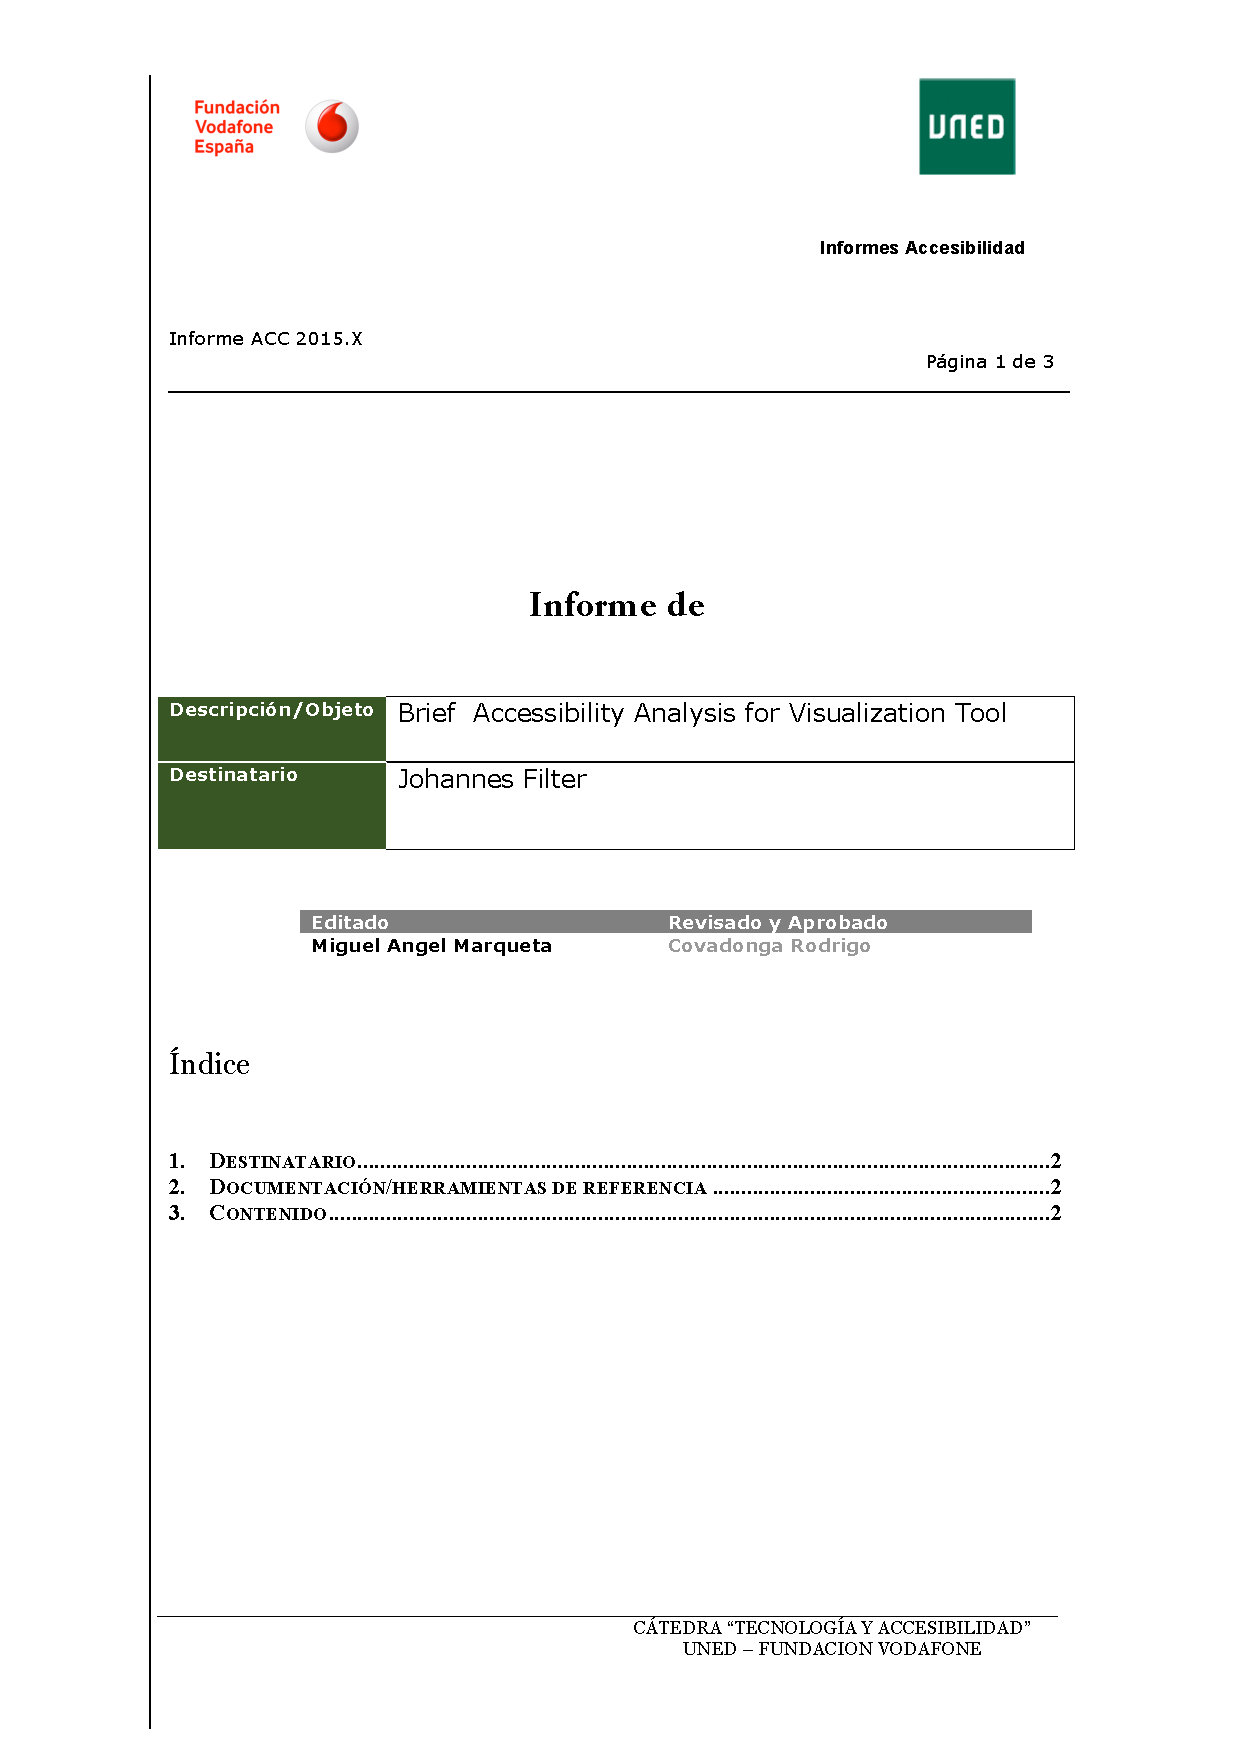
\includepdf[pages={-}]{appendix/report.pdf}

\chapter{Appendix: Closed Questions}
\label{app:closed}

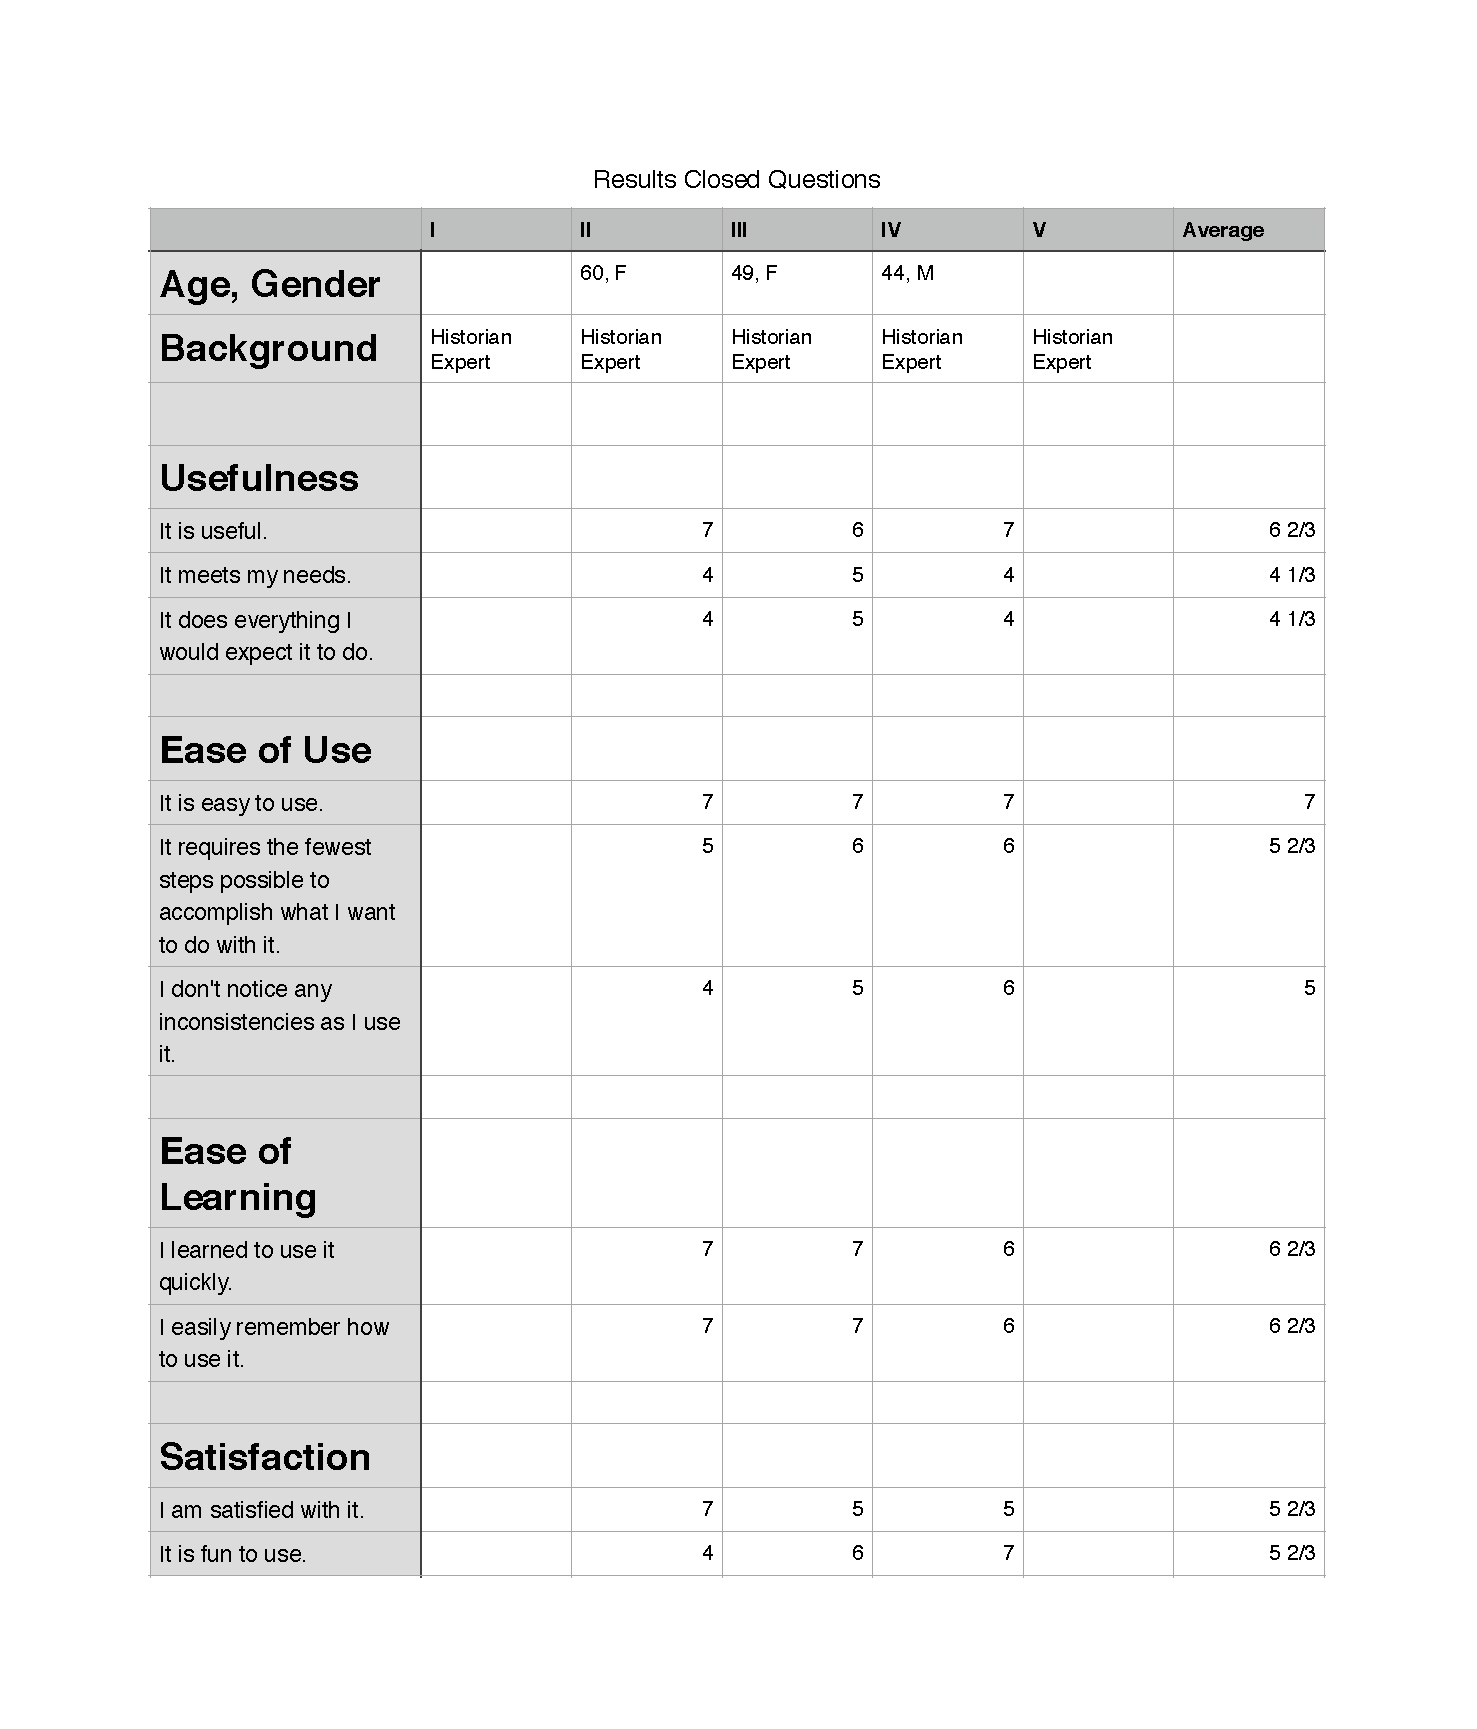
\includepdf[pages={-}]{appendix/closed.pdf}

\chapter{Appendix: Open Questions}
\label{app:open}

\begin{itemize}
	\item What were the most positive things about using this system and why?
	\item What were the most negative things about using this system and why?
	\item How would you improve this system and why?
	\item Is there anything else that you would like to tell us about this system and your experiences using it?
	\item In comparison with other systems (Interface of Catálogo Colectivo de las colecciones de Mapas and previous work of this research group).
Do you think it is more useful? If yes, which part of the system is more useful.
\end{itemize}


\end{document}